\RequirePackage[hyphens]{url}
\documentclass{sig-alternate}

\hyphenation{data-bases}

\newcommand{\TITLE}{Evaluating the Scientific Impact of XSEDE}
\newcommand{\AUTHOR}{Fugang Wang, Gregor von Laszewski}

%%%%%%%%%%%%%%%%%%%%%%%%%%%%%%%%%%%%%%%%%%%%%%%%%%%%%%%%%%%%%%
% LATEX DEFINITIONS 
%%%%%%%%%%%%%%%%%%%%%%%%%%%%%%%%%%%%%%%%%%%%%%%%%%%%%%%%%%%%%%

\usepackage{float}
\usepackage{comment}
\usepackage{hyperref} 
\usepackage{array} 
\usepackage{graphicx} 
\usepackage{booktabs} 
\usepackage{pifont} 
\usepackage{todonotes} 
\usepackage{rotating} 
\usepackage{color} 
\usepackage{caption}
\captionsetup{font={scriptsize}}

\newcommand*\rot{\rotatebox{90}} 

\newcommand{\FILE}[1]{\todo[color=green!40]{#1}} 

%
% more floats on one page
%
\renewcommand{\topfraction}{.85}
\renewcommand{\bottomfraction}{.7}
\renewcommand{\textfraction}{.15}
\renewcommand{\floatpagefraction}{.66}
\renewcommand{\dbltopfraction}{.66}
\renewcommand{\dblfloatpagefraction}{.66}
\setcounter{topnumber}{9}
\setcounter{bottomnumber}{9}
\setcounter{totalnumber}{20}
\setcounter{dbltopnumber}{9}

%%%%%%%%%%%%%%%%%%%%%%%%%%%%%%%%%%%%%%%%%%%%%%%%%%%%%%%%%%%%%%
% HYPERSETUP 
%%%%%%%%%%%%%%%%%%%%%%%%%%%%%%%%%%%%%%%%%%%%%%%%%%%%%%%%%%%%%%

\hypersetup{ 
    bookmarks=true,         % show bookmarks bar 
    unicode=false,          % non-Latin characters in Acrobat's bookmarks 
    pdftoolbar=true,        % show Acrobat's toolbar 
    pdfmenubar=true,        % show Acrobat's menu 
    pdffitwindow=false,     % window fit to page when opened 
    pdfstartview={FitH},    % fits the width of the page to the window 
    pdftitle={\TITLE},    % title 
    pdfauthor={\AUTHOR},     % author 
    pdfsubject={Subject},   % subject of the document 
    pdfcreator={Gregor von Laszewski, Fugang Wang},   % creator of the document 
    pdfproducer={}, % producer of the document 
    pdfkeywords={bibliometrics} {hindex} {XSEDE} {FWCI}, % list of keywords 
    pdfnewwindow=true,      % links in new window 
    colorlinks=true,     % false: boxed links; true: colored links 
    linkcolor=black,     % color of internal links (change box color with linkbordercolor) 
    citecolor=black,     % color of links to bibliography 
    filecolor=black,     % color of file links 
    urlcolor=black       % color of external links 
} 

\begin{document}


\conferenceinfo{PEARC18 ...}{2018,USA}
\CopyrightYear{2018} 
\crdata{TBD...\$15.00.\\
http://dx.doi.org/TBD
} 

\title{\TITLE\vspace{-12pt}}

\numberofauthors{6}  
\author{ 
\alignauthor 
Fugang Wang\\
       \affaddr{Indiana University}\\ 
       \affaddr{Bloomington, Indiana, U.S.A.}\\ 
\alignauthor
Gregor von Laszewski\titlenote{Corresponding Author.}\\
       \affaddr{Indiana University}\\ 
       \affaddr{Bloomington, Indiana, U.S.A.}\\ 
       \email{laszewski@gmail.com}
\alignauthor
Timothy Whitson\\
       \affaddr{Indiana University}\\ 
       \affaddr{Bloomington, Indiana, U.S.A.}\\ 
\and
\alignauthor
Geoffrey C. Fox\\
       \affaddr{Indiana University}\\ 
       \affaddr{Bloomington, Indiana, U.S.A.}\\ 
\alignauthor  
Thomas R. Furlani\\
       \affaddr{Center for Computational Research}\\
       \affaddr{University at Buffalo, SUNY}\\ 
       \affaddr{701 Ellicott Street}\\ 
       \affaddr{Buffalo, New York, 14203}
\alignauthor  
Robert L. DeLeon\\
Steven M. Gallo\\
       \affaddr{University at Buffalo, SUNY}\\ 
       \affaddr{Buffalo, New York, 14203}
}

\date{July 2018}

\maketitle

\begin{abstract}

  We use the bibliometrics approach to evaluate the scientific impact of
  XSEDE.  By utilizing publication data from various sources, e.g.,
  ISI Web of Science and Microsoft Academic Graph, we calculate the
  impact metrics of XSEDE publications and show how they compare with
  non-XSEDE publication from the same field of study, or non-XSEDE
  \emph{peers} from the same journal issue. We explain in detail how
  we retrieved, cleaned, and curated millions of related publication
  entries.  We then introduce the metrics we used for evaluation and
  comparison, and the methods used to calculate them. Detailed
  analysis results of Field Weighted Citation Impact (FWCI) and the
  peers comparison will be presented and discussed. We also explain
  how the same approaches could be used to evaluate publications from
  a similar organization or institute, to demonstrate the general
  applicability of the present evaluation approach providing impact
  even beyond XSEDE.


\end{abstract}


\vspace{-6pt}

\category{H.4}{Information Systems Applications}{Miscellaneous}
\category{D.2.8}{Software Engineering}{Metrics}[complexity measures,
performance measures]

\terms{Theory, Measurement}

\keywords{Scientific impact, bibliometrics, h-index, Technology Audit
  Service, XDMoD, XSEDE}

\section{Introduction} 

To identify the impact of {\em scientific advancements enabled by
  enhanced cyberinfrastructure}, it is important to conduct a
comprehensive analysis of achievements that can be attributed to the
use of the advanced infrastructure, such as that provided by the
Extreme Science and Discovery Environment
(XSEDE)~\cite{www-xsede,xsede}.

We use the bibliometrics approach to evaluate the scientific impact of
XSEDE. By acquiring related publication and citation data from
multiple sources we calculate various metrics that show the impact of
the publications and how they compare to their non-XSEDE peers that
were published in the same journals, or in the same field of study. By
processing millions of publication data entries we normalized the
citation count by field of study. This essentially eliminates the
problem that different fields of study have different publication
characteristics. We introduced a novel \cite{tas2015} method to compare the
target publications group with their peers published in the same
publication venue to further show how the target publications group
performs compared to their peers within the same publication venue.


\section{Related Works} \label{S:related}

Bibliometrics based analysis has been the most commonly used method to
evaluate the research impact of an individual, a research group, or
even an organization. Publication count and citation count based
metrics provide an effective way to show the quantity and quality, and
the impact of scientific research activities. For instance, it was
used to evaluate the quality of research in the United
Kingdom~\cite{thomas1998institutional,penfield2014assessment}. Most
popular college/university rankings use citation based bibliometrics
as an important factor to evaluate the quality of their research,
e.g., the overall publication count and citation count in a certain
year or a year range; the number of papers published in certain top
journals; the number of highly cited papers; rating the citation count
of a paper or its percentile ranking, etc.

Compute Canada, a virtual organization similar to XSEDE, also uses a
bibliometrics based analysis to evaluate the impact of their
research~\cite{www-computecanada}.

Some previous limited work studied the impact of
TeraGrid~\cite{bollen2011and}, the early version of XSEDE, by
analyzing the publications for one specific research allocation
quarter, which involved a very limited number of researchers and
publications. Our work is unique in that it provides a {\em
  comprehensive} analysis superior in data volume, and with novel
analyses approach such as Field Weighted Citation Impact and journal
publication-based peers comparison.

In addition to the more intuitive direct metrics of publication and
citation count, some other derivative metrics such as
h-index~\cite{hirsch2005index} and g-index~\cite{egghe2006theory}
combines both publication and citation count to generate one
metric. I10-index~\cite {www-i10index} in contrast measures only the
count of those publications that received at least ten references by
other publications.  In our evaluation we calculated such metrics for
various XSEDE research entities to show the impact and comparison of
the entities on the same level, e.g., individual, project, research
field of study, organization, etc. The results are presented on the
XDMoD scientific impact portal~\cite{www-xdmod-sciimp}.


Usage based
metrics~\cite{Bollen:2007:MUM:1255175.1255273,Bollen:2008:TUI:1378889.1378928}
have also been proposed including metrics such as views and downloads,
instead of the more formal citations of publications. However the
applicability of this approach may be limited because the usage data
may not be available from a publisher, or different publishers may
have different criteria to measure the usage data. Thus, it would
create an inconsistent comparison for papers published by different
publishers.  For this reason we did not present such metrics in this
paper.

\section{Methodology} \label{S:methodology}

We first introduce the methodology we use in the bibliometrics
analysis to evaluate the scientific impact of XSEDE publications. This
includes the specification of the dataset and data sources used in the
analysis, the approaches to define and calculate the various metrics,
and the information about the sophisticated software and service
framework developed to facilitate this to XSEDE unique and
comprehensive evaluation study.

\subsection{Dataset and data sources}

Several data sets and sources are involved in this study which
includes XSEDE publications, Microsoft Academic Graph (MAG), and Web
of Science Data. For all data we used the same time period between
2005 and 2016, which is the same as for the XSEDE publications. We
describe the basic features of the datasets next.

\parindent 0pt \textbf{XSEDE publications} include those from
TeraGrid. This data is collected from two sources. One is from the
user-submitted data from the XSEDE user portal; another is from the
past TeraGrid/XSEDE project reports submitted to NSF. For the latter,
we extracted the publications appendix from the reports and then
parsed and curated with significant effort the publication records
text, before putting them into a structured database. There were over
20 thousand raw entries.

\parindent 0pt \textbf{Microsoft Academic Graph (MAG)} This dataset
was retrieved with the API provided by Microsoft. The data was then
curated and cleaned and put into a MongoDB database. This dataset has
about 58 million entries.

\parindent 0pt \textbf{ISI Web of Science (WoS)} is used for the publication
venues with at least 10 XSEDE papers appearing in them to facilitate
the peers comparison study. This dataset has about 2 million entries.

\subsection{Field Weighted Citation Impact Analysis}

The field Weighted Citation Impact (FWCI) metric is proposed as one of
the snowball metrics~\cite{colledge2014snowball}. It calculates the
average citation count of a target group of publications based on
their field of science, and then compare that with the average
citation count of the whole field of science in the same time
period. The result is a ratio

\[ FWCI = avg(CC_{group})/avg(CC_{field}) \]

A \emph{FWCI} value greater than 1 indicates that the pertinent
publication group had more citations than the expected value of the
field of science, while a value less than 1 indicates that the average
citation count that the group received was less than the expected
value for the applicable field of science.

In this study we introduced the following process to calculate the \emph{FWCI}
values for the XSEDE publications.

\begin{enumerate}
\item Query every raw XSEDE publication by title against the MAG data
  set, and verify the matching ones by checking other properties such
  as published year. After this process we identify the verified
  matching records in the MAG for all valid XSEDE publications.
  During this process we use elasticsearch
  \cite{gormley2015elasticsearch} to improve both the accuracy and the
  performance of the query.  This is important because of the size of
  the dataset.
\item For each of the 58 million MAG data records, we use the assigned
  field of study values, along with other related data form MAG, to
  \emph{trace} upward to the top levels of the hierarchical
  fields. This process narrowed down the ~30k different assigned
  fields of study to 19 overall top level \emph{fields of study} as
  defined in the MAG dataset.  One thing to note is that each
  publication is assigned to multiple science fields in the original
  publication records, and the final top level science field category
  of a publication may not be unique either. However as a lot of
  research publications are themselves multi-disciplinary we think
  that such results are valid and acceptable.

  In the following analysis we counted a publication in all the top
  level science fields that we found following this tracing process.

\item Once we have each and every publications in the MAG dataset, we
  can calculate the average citation count by each top level field,
  for all the MAG publications and XSEDE publications
  respectively. Following that we can calculate the ratio to get the
  FWCI values.
\end{enumerate}

\subsection{Metric for Journal Publication-based Peer Comparison} \label{S:metric}

An importnat achievement is our novel and sophisticated \emph{Journal
  Publication-based Peer Comparison (JPPC)} metric as discussed in
\cite{tas2015}. We used the following process to obtain the data
needed for the analysis.

\begin{enumerate}
\item We start this analysis by querying all XSEDE publications
  against a third party data source - WoS~\cite{www-isiwos}. The XSEDE
  data, as explained before, contains the publication entries
  extracted from past TeraGrid/XSEDE reports to NSF, and the
  publication data from the XSEDE user portal. Both are user-submitted
  data or compiled from user-submitted data, thus this query and
  verification process is needed to ensure the quality and accuracy of
  the dataset.  This resulted in about nine thousand verified
  publications at the time of the study.

\item From this verified publications list, we find the subset of all
  publication venues with at least 10 XSEDE publications. For each of
  the publications published in these venues we retrieve from WoS the
  extended metadata to get the exact volume and issue number of the
  publication venue. The reasons why we chose a threshold value of 10
  to identify a publication venue subset are:

  \begin{enumerate}
  \item This ensures the statistical significance of the analysis
    results.
  \item This eases the data retrieval work substantially. While we
    have \verb|~|1400 distinct publication venues identified from all the
    verified XSEDE publications, the subset when we use 10 as the
    minimum number of publications appearing in the venue was reduced
    to \verb|~|120 publication venues.
  \item Using this criterion, the number of XSEDE publications in the
    peers comparison was about five thousand, or about 56\% of all the
    verified ones. This represents a good portion of all the data.
  \end{enumerate}

\item For all \verb|~|120 publication venues, we retrieved all the
  publications data published in them during the same time period as
  the TeraGrid/XSEDE publications (2005-2016).
\end{enumerate}

Based on this data, we can establish suitable comparison peer groups,
which are based each on a single journal issue (or journal volume when
no issue data available for some publications) that an XSEDE
publication appeared in. For each comparison peer group, we rank the
citation count of each publication (including the XSEDE ones and the
peers). The calculated percentile ranking values serve as the basis of
the peer comparison study. The comparison is between publications that
we identified as XSEDE papers and those that were not.

To apply the percentile ranking to the field of science of XSEDE
publications among the journal issues where each publication was
published, we aggregate them based on the project field
of science data obtained from the XSEDE central database
(XDcDB). These XSEDE fields of science are self-reported by the
researchers. We then calculate the average and median percentile rank
for each field of science (FOS).

\begin{comment}
To identify the FOS for each publication, we followed this process:

\begin{enumerate}

\item Find the FOS information for each publication out of the past
  XSEDE quarterly reports as this information may have been explicitly
  associated with the publication.

\item Find the FOS information from the project data in the
  XDcDB. Similar to the case mentioned in MAG data pre-processing, it
  is possible that one project is associated with more than one
  FOS. In such cases we counted the publications of the project for
  all involved fields.

  \begin{enumerate}

  \item Some publications from the XSEDE quarterly reports were
    identified only by the project proposal number. We mapped them to
    the project charge number and account id used internally within
    the XSEDE central database.

  \item For user uploaded publications data via the XSEDE user portal,
    a project charge number was associated with each publication.

  \item Identify from the charge number the FOS as defined in the
    XDcDB.

  \end{enumerate}

\end{enumerate}
\end{comment}

\subsection{Software Architecture Supporting the Study}

We have developed a sophisticated software framework supporting the
study, which includes data acquisition, cleanup, processing and
presentation. The framework is based on a distributed set of software
services. This service-oriented framework is integrated as part of a
layered architecture consisting of components for:

\begin{itemize}
\item A data layer that retrieves publication and citation data from
  external sources.  This includes data from the ISI Web of Knowledge;
  Microsoft Academic Graph; Google Scholar, and very importantly the
  NSF award database.

\item Business logic layer that deals with:

  \begin{itemize}
  \item parsing and processing while correlating data from various
    databases and services, such as the XSEDE central database
    (XDcDB).
  \item a metrics generation and analysis system for different
    aggregation levels -- users, projects, organization, field of
    science.
  \end{itemize}

\item a presentation layer using a lightweight portal in addition to
  exposing some data via a RESTful API
  ~\cite{Wang:2014:TSI:2616498.2616507}.
\end{itemize}

Due to the use of the Software as a Service (SaaS) approach, our
framework is \emph{expandable} as we are able to integrate new
services and data resources as required. Hence our framework can be
adapted to other resource providers as demonstrated
in~\cite{tas2015}. Obviously, adaptation could mean that we have to
change the bibliometric data, which could mean that we need to
integrate new data sources and curation services spending significant
effort to integrate such data.

\subsubsection{Service Integration into XSEDE and XDMoD}

Our current framework for XSEDE includes services that are motivated
by our initial findings from the XSEDE bibliometric data. A RESTful
service is integrated into the \emph{XSEDE User Portal} as part of the
publication discovery service.

The various impact metrics of different levels of XSEDE entities -
person, project, organization, field of study - as well as part of the
analyses are available on the \emph{XDMoD scientific impact
portal}~\cite{www-xdmod-sciimp}.

\section{Results and Discussions} \label{S:result}

In this paper, we discuss results specifically targeting the analysis
of data related to XSEDE.

\subsection{Field Weighted Citation Impact Metrics}

First we show the calculated FWCI values in
Figure~\ref{F:fwci_fwci}. The plot lists the FWCI for the top-level
fields of science as defined from the MAG data.  Each data point also
has the number of XSEDE publications as well as the number of all
publications in that field. The red vertical line indicates the point
at which FWCI=1. Figure~\ref{F:fwci_fwci} shows all fields but one
(political science, with only 3 publications) that had FWCI values
greater than 1, with the majority fields having much higher values.

In Figure \ref{F:fwci_nxd} we display the same data but sort it based
on the number of XSEDE publications in the field. This emphasizes the
FWCI for the fields that the majority of the XSEDE publications fell
within.

\begin{figure}[htb!]
  \centering
    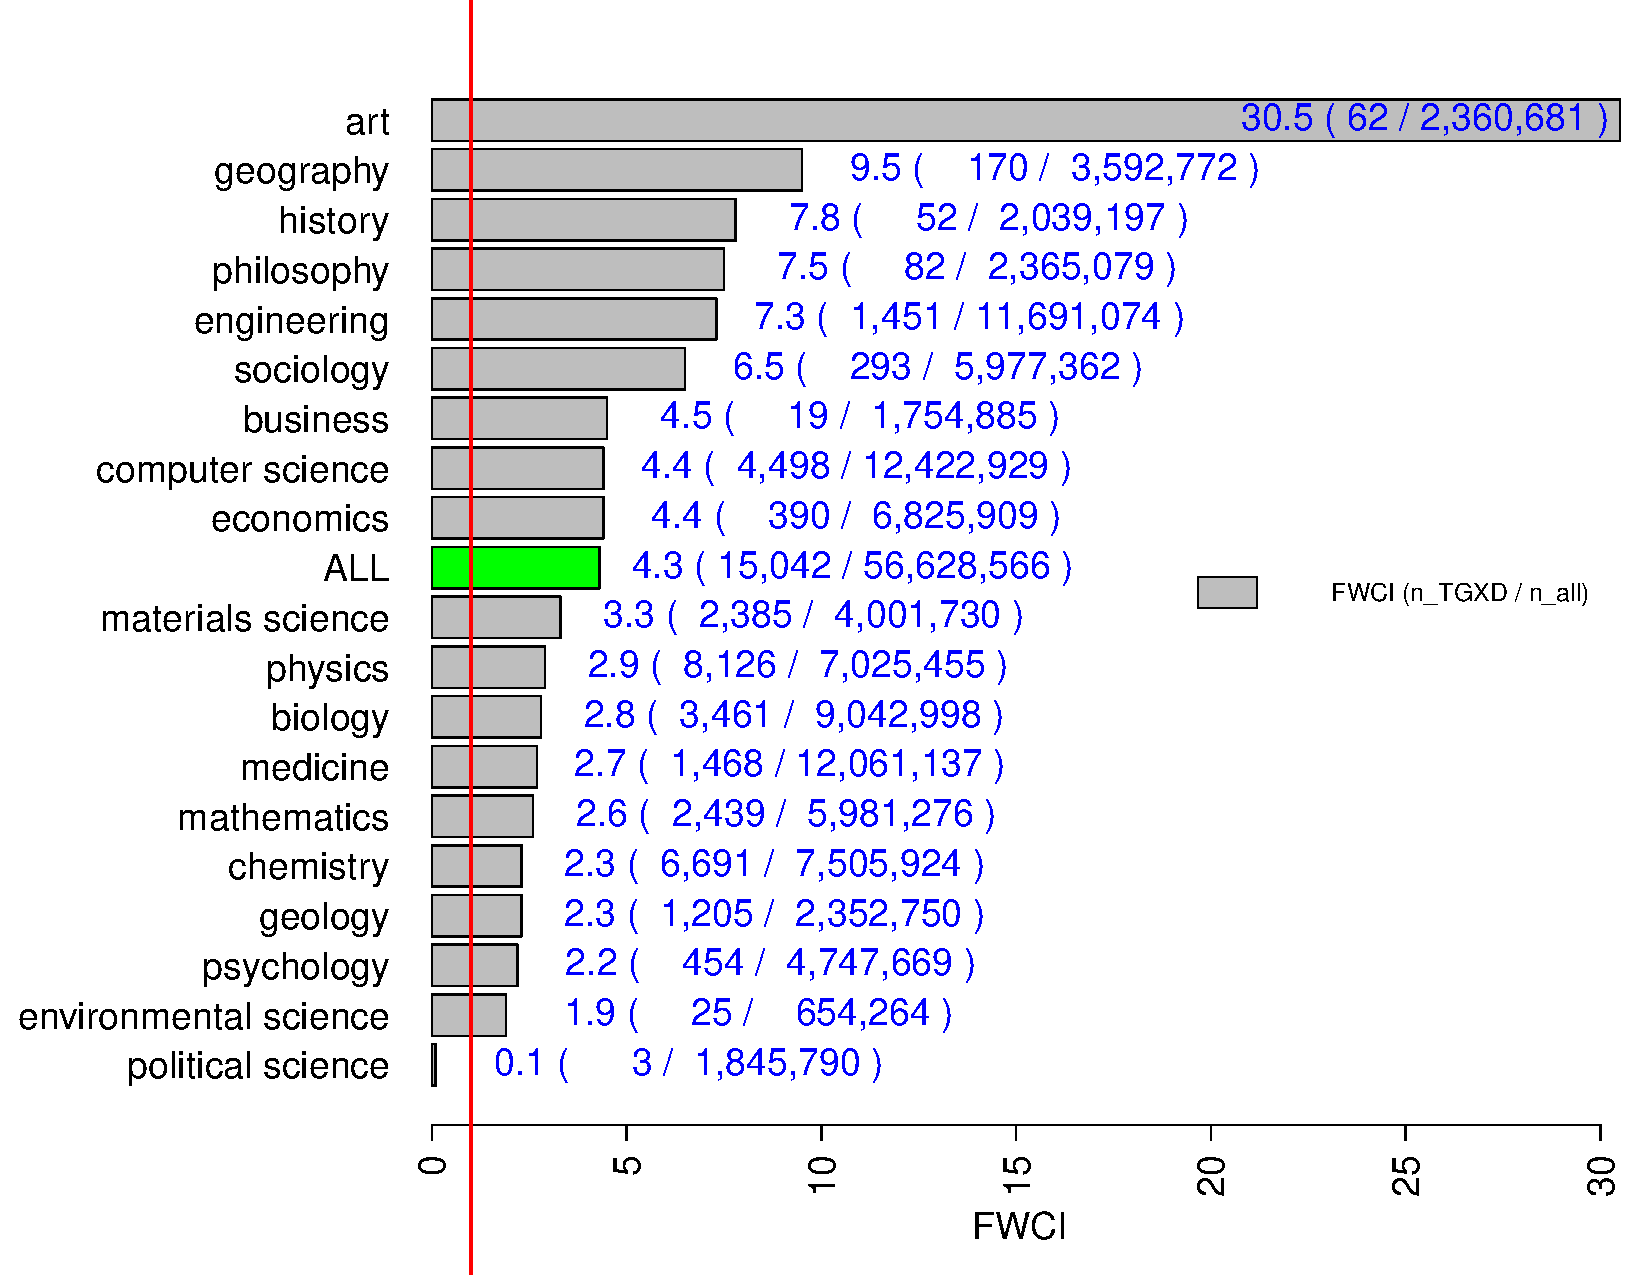
\includegraphics[width=0.95\columnwidth]{images/fwci_fwci.pdf}
    \caption{Field Weighted Citation Impact (FWCI) by Field sorted by FWCI.}
    \label{F:fwci_fwci}
\end{figure}

\begin{figure}[htb!]
  \centering
    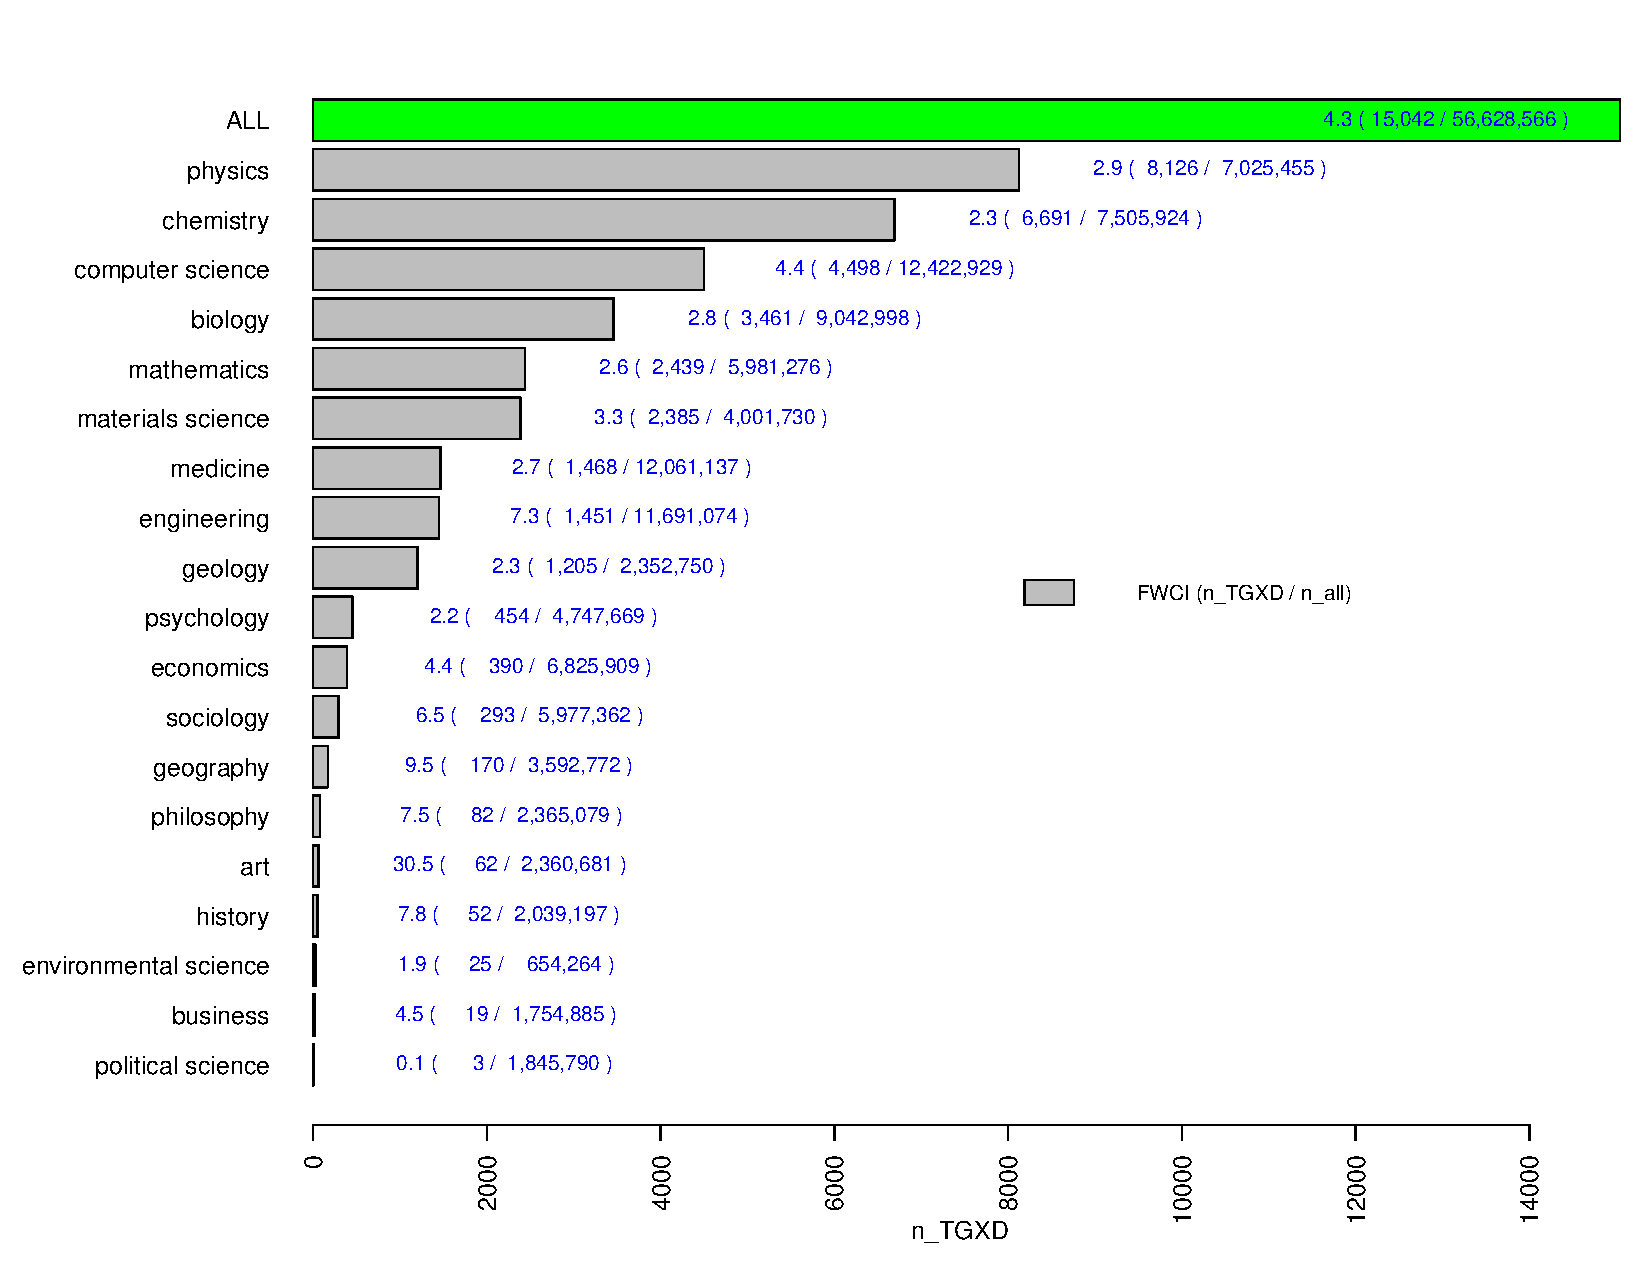
\includegraphics[width=0.95\columnwidth]{images/fwci_nxd.pdf}
    \caption{FWCI by Field sorted by Publication Count of the Field.}
    \label{F:fwci_nxd}
\end{figure}

Figure \ref{F:FWCIwCC} compares the expected citation count based on
all publications in a given field of science with the actual average
citation count for XSEDE publications in each field of science, while
including the FWCI values at the same time. The plot was sorted based
on the number of XSEDE publications in the field. This
again indicates that XSEDE publications received much higher citation
counts and implies a higher scientific impact than their non-XSEDE
peers.

In Figure~\ref{F:FWCI_CC} we show the extra citations XSEDE
publications receive for each field, compared to the expected overall
field of science value. Figure~\ref{F:FWCI_CC} also indicates how much
impact that access to XSEDE resources has on each individual field of
science.

\begin{figure}[htb!]
  \centering
    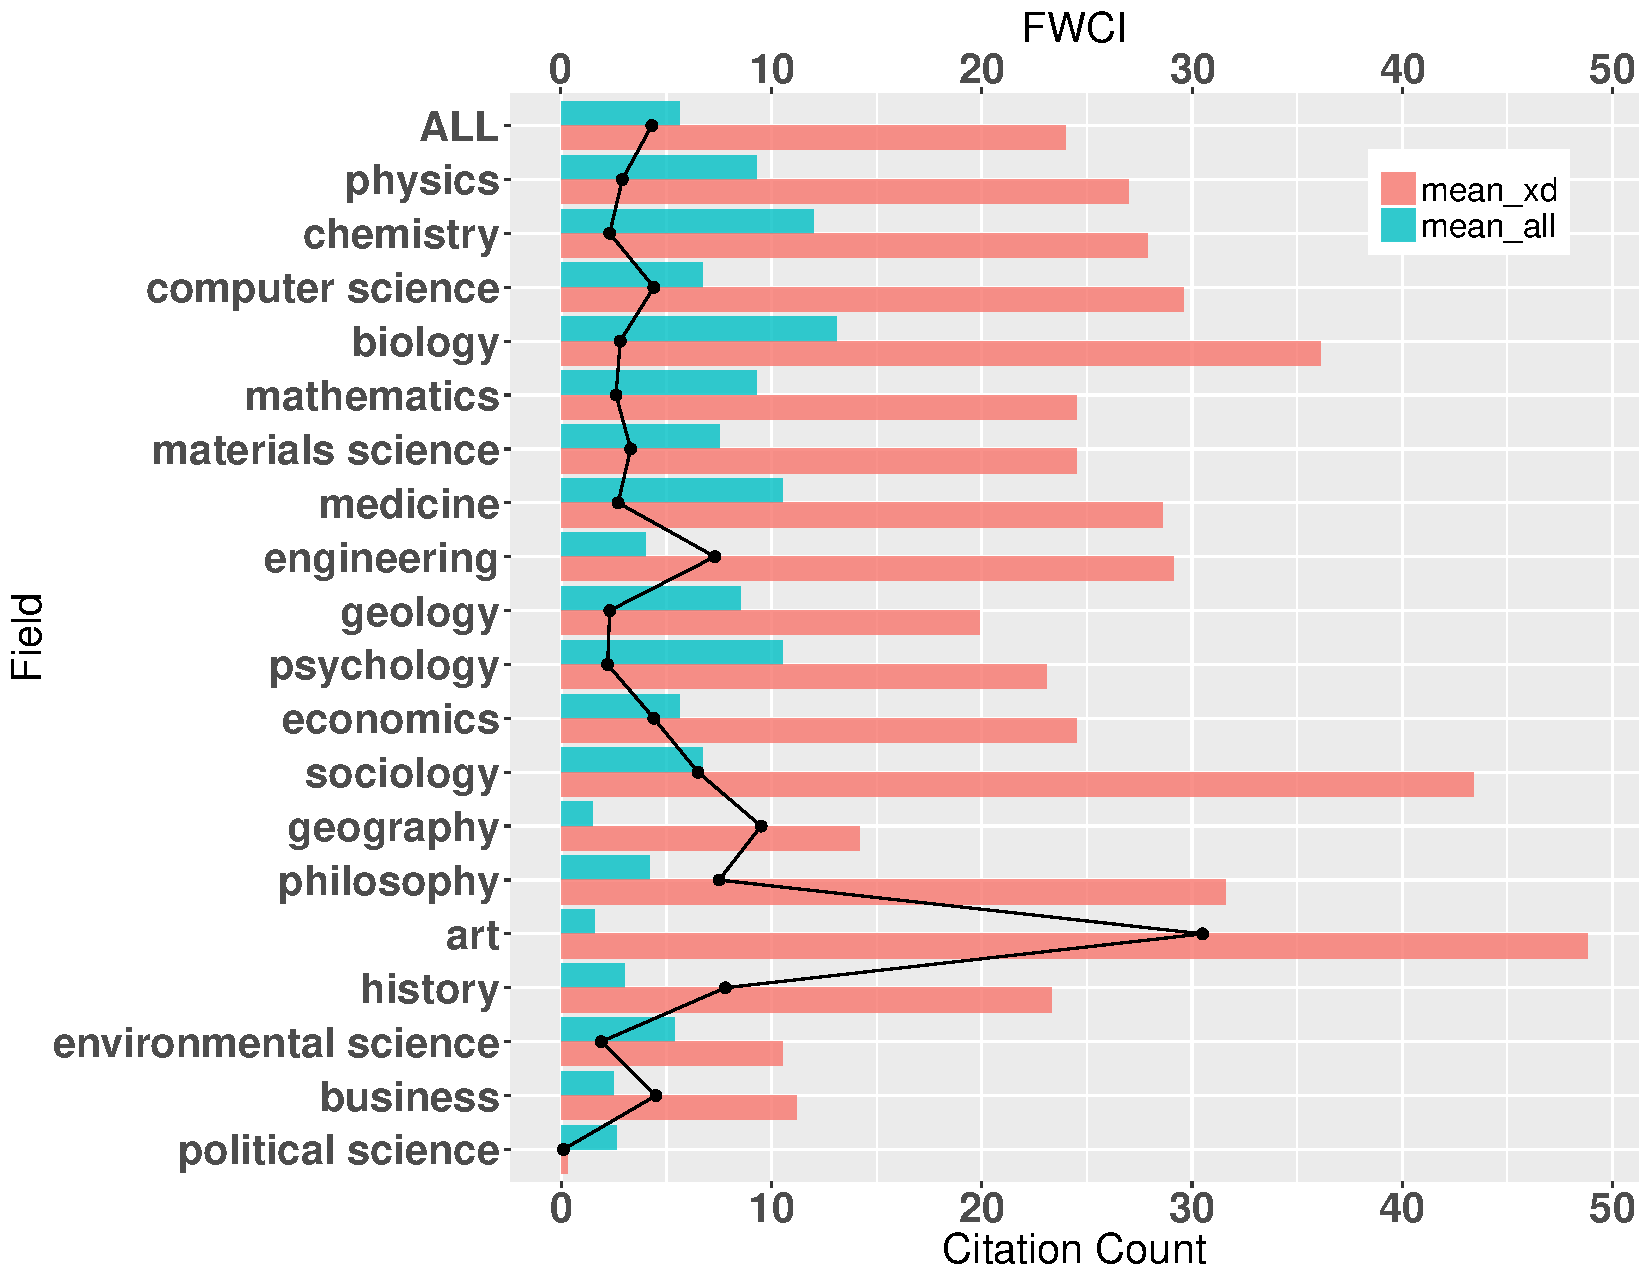
\includegraphics[width=0.95\columnwidth]{images/FWCIwCC.pdf}
    \caption{FWCI with Expected Citation Count and Actual Citation Count from XD Publications.}
    \label{F:FWCIwCC}
\end{figure}

\begin{figure}[htb!]'
  \centering
    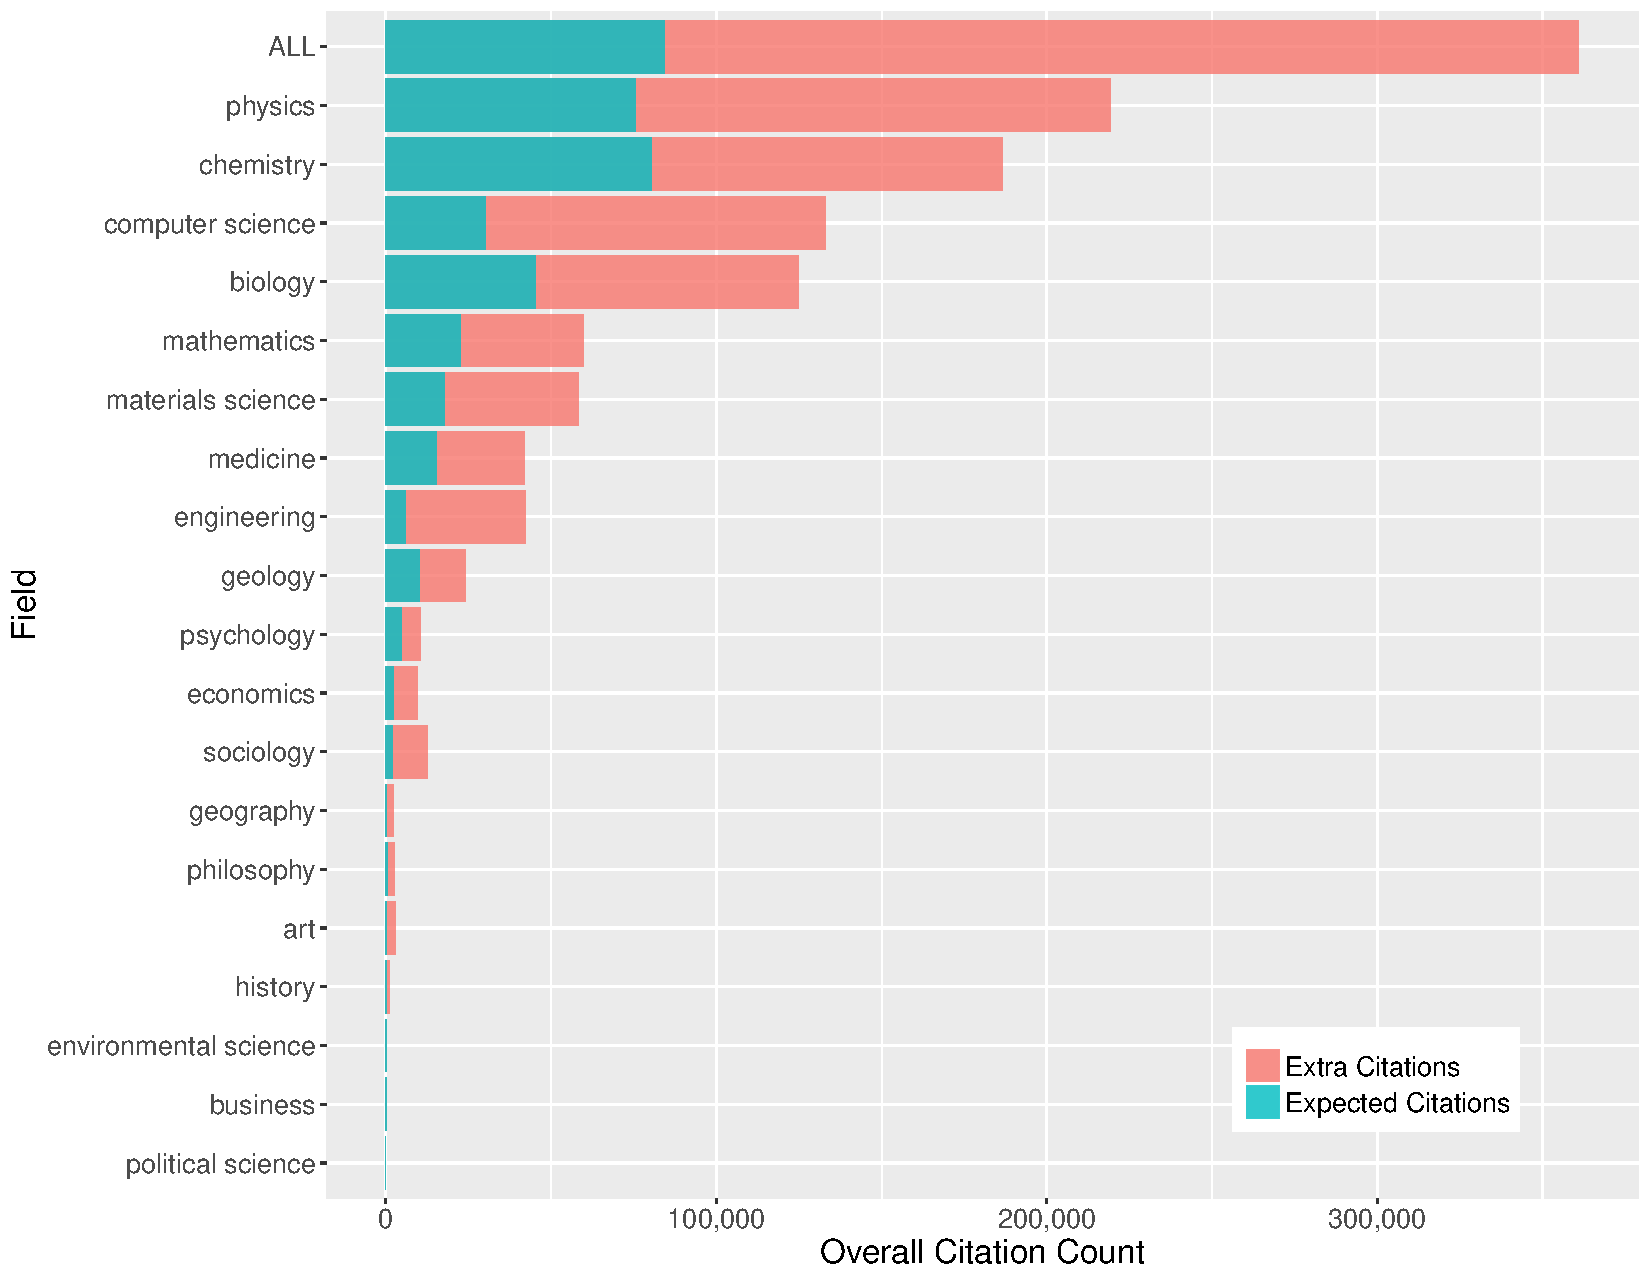
\includegraphics[width=0.95\columnwidth]{images/FWCI_CC.pdf}
    \caption{Extra Citation Count Achieved by XD Publications.}
    \label{F:FWCI_CC}
\end{figure}

The availability of all the publications for each field makes it
possible to calculate other interesting statistics, in addition to the
above presented FWCI results. In Table \ref{T:field_highly_cited} we
display for each field the highly cited XSEDE papers (defined as top
1\% and top 5\% in citation count in that field) and the percentage of
how many XSEDE publications fall into each category. The results show
that for most fields a higher than expected percentage of XSEDE
publications fall into the highly cited papers categories. E.g., when
we consider all the publications and fields together, 4.8\% XSEDE
publications were in the top 1\% highly cited group while 22.5\% were
in the top 5\% highly cited group.

\begin{table*}[t]
\caption{Highly Cited Papers Statistics (in top 1\% and 5\%)}
\label{T:field_highly_cited}
\centering
\resizebox{0.75\textwidth}{!}{%
 \begin{tabular}{||c c c c c c c||}
 \hline
Field &    \# in top 1\% & \% in top 1\% & \# in top 5\% & \% in top 5\% & \# per 100,000 & \# XSEDE pubs \\ [0.5ex]
 \hline\hline
ALL & 727 & 4.8 & 3380 & 22.5 & 26.6 & 15042 \\
\hline
physics & 292 & 3.6 & 1204 & 14.8 & 115.7 & 8126 \\
\hline
chemistry & 177 & 2.6 & 782 & 11.7 & 89.1 & 6691 \\
\hline
computer science & 223 & 5.0 & 1037 & 23.1 & 36.2 & 4498 \\
\hline
biology & 102 & 2.9 & 453 & 13.1 & 38.3 & 3461 \\
\hline
mathematics & 68 & 2.8 & 351 & 14.4 & 40.8 & 2439 \\
\hline
materials science & 108 & 4.5 & 446 & 18.7 & 59.6 & 2385 \\
\hline
medicine & 42 & 2.9 & 213 & 14.5 & 12.2 & 1468 \\
\hline
engineering & 111 & 7.6 & 414 & 28.5 & 12.4 & 1451 \\
\hline
geology & 33 & 2.7 & 183 & 15.2 & 51.2 & 1205 \\
\hline
psychology & 11 & 2.4 & 53 & 11.7 & 9.6 & 454 \\
\hline
economics & 26 & 6.7 & 101 & 25.9 & 5.7 & 390 \\
\hline
sociology & 18 & 6.1 & 63 & 21.5 & 4.9 & 293 \\
\hline
geography & 19 & 11.2 & 87 & 51.2 & 4.7 & 170 \\
\hline
philosophy & 11 & 13.4 & 31 & 37.8 & 3.5 & 82 \\
\hline
art & 15 & 24.2 & 39 & 62.9 & 2.6 & 62 \\
\hline
history & 6 & 11.5 & 19 & 36.5 & 2.6 & 52 \\
\hline
environmental science & 1 & 4.0 & 3 & 12.0 & 3.8 & 25 \\
\hline
business & 1 & 5.3 & 6 & 31.6 & 1.1 & 19 \\
\hline
political science & 0 & 0.0 & 0 & 0.0 & 0.2 & 3 \\ [1ex]
 \hline
\end{tabular}
}
\end{table*}

\subsection{XSEDE Peer Data Analysis} \label{S:xsede}

Now we present a number of graphs and tables that show the results
from the peer comparison study. Figure \ref{F:isi_peers_byj_mean}
shows the average percentile rank of XSEDE publications grouped by
each publication venue. Figure \ref{F:isi_peers_byj_median} shows the
same publication data but presents the median percentile rank values.

\begin{figure*}[htb!]
  \centering
    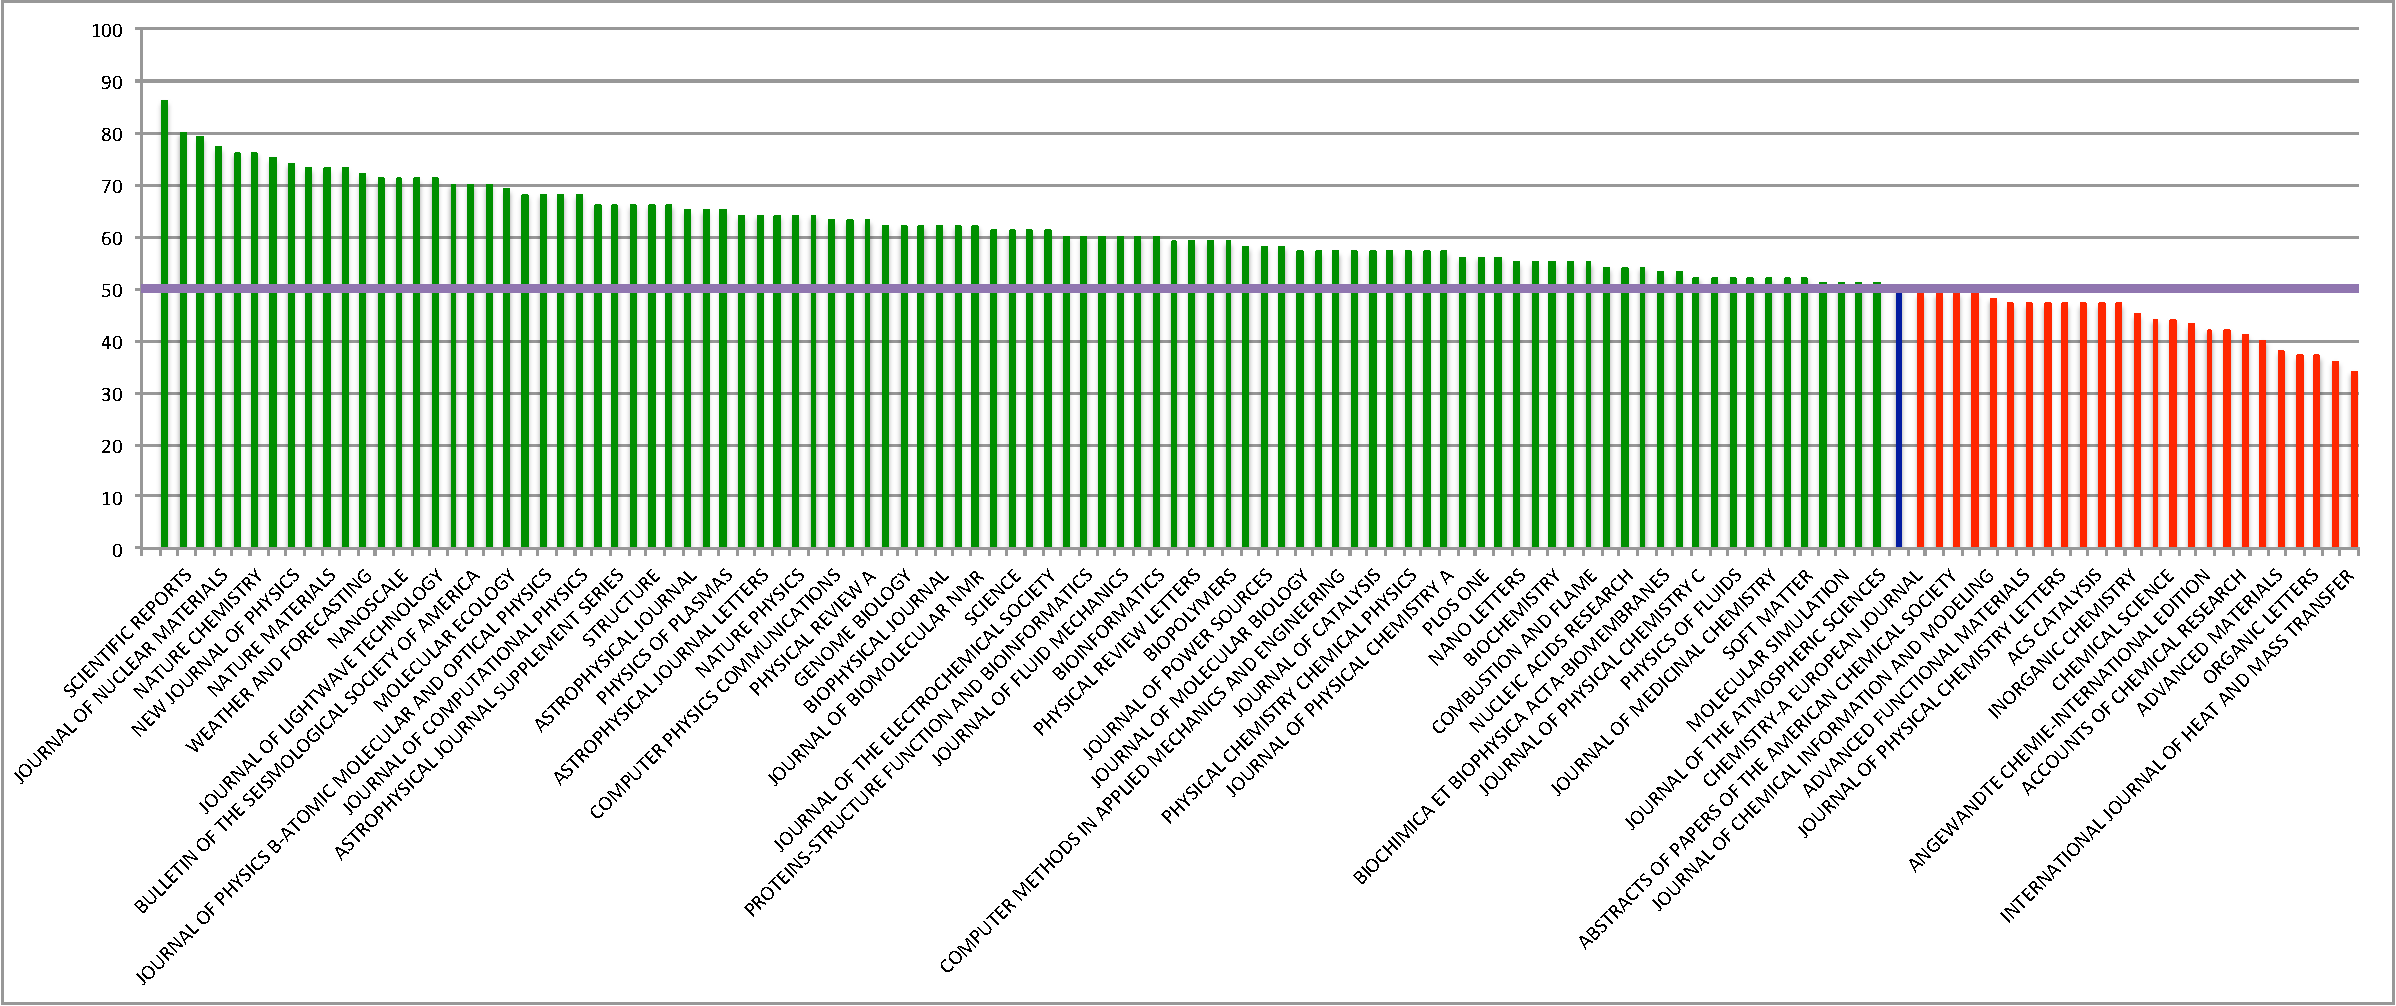
\includegraphics[width=0.9\textwidth]{images/isi_peers_byj_mean.pdf}
    \caption{Average percentile ranking of XD publications by journal (by ISI)}
    \label{F:isi_peers_byj_mean}
\end{figure*}

\begin{figure*}[htb!]
  \centering
    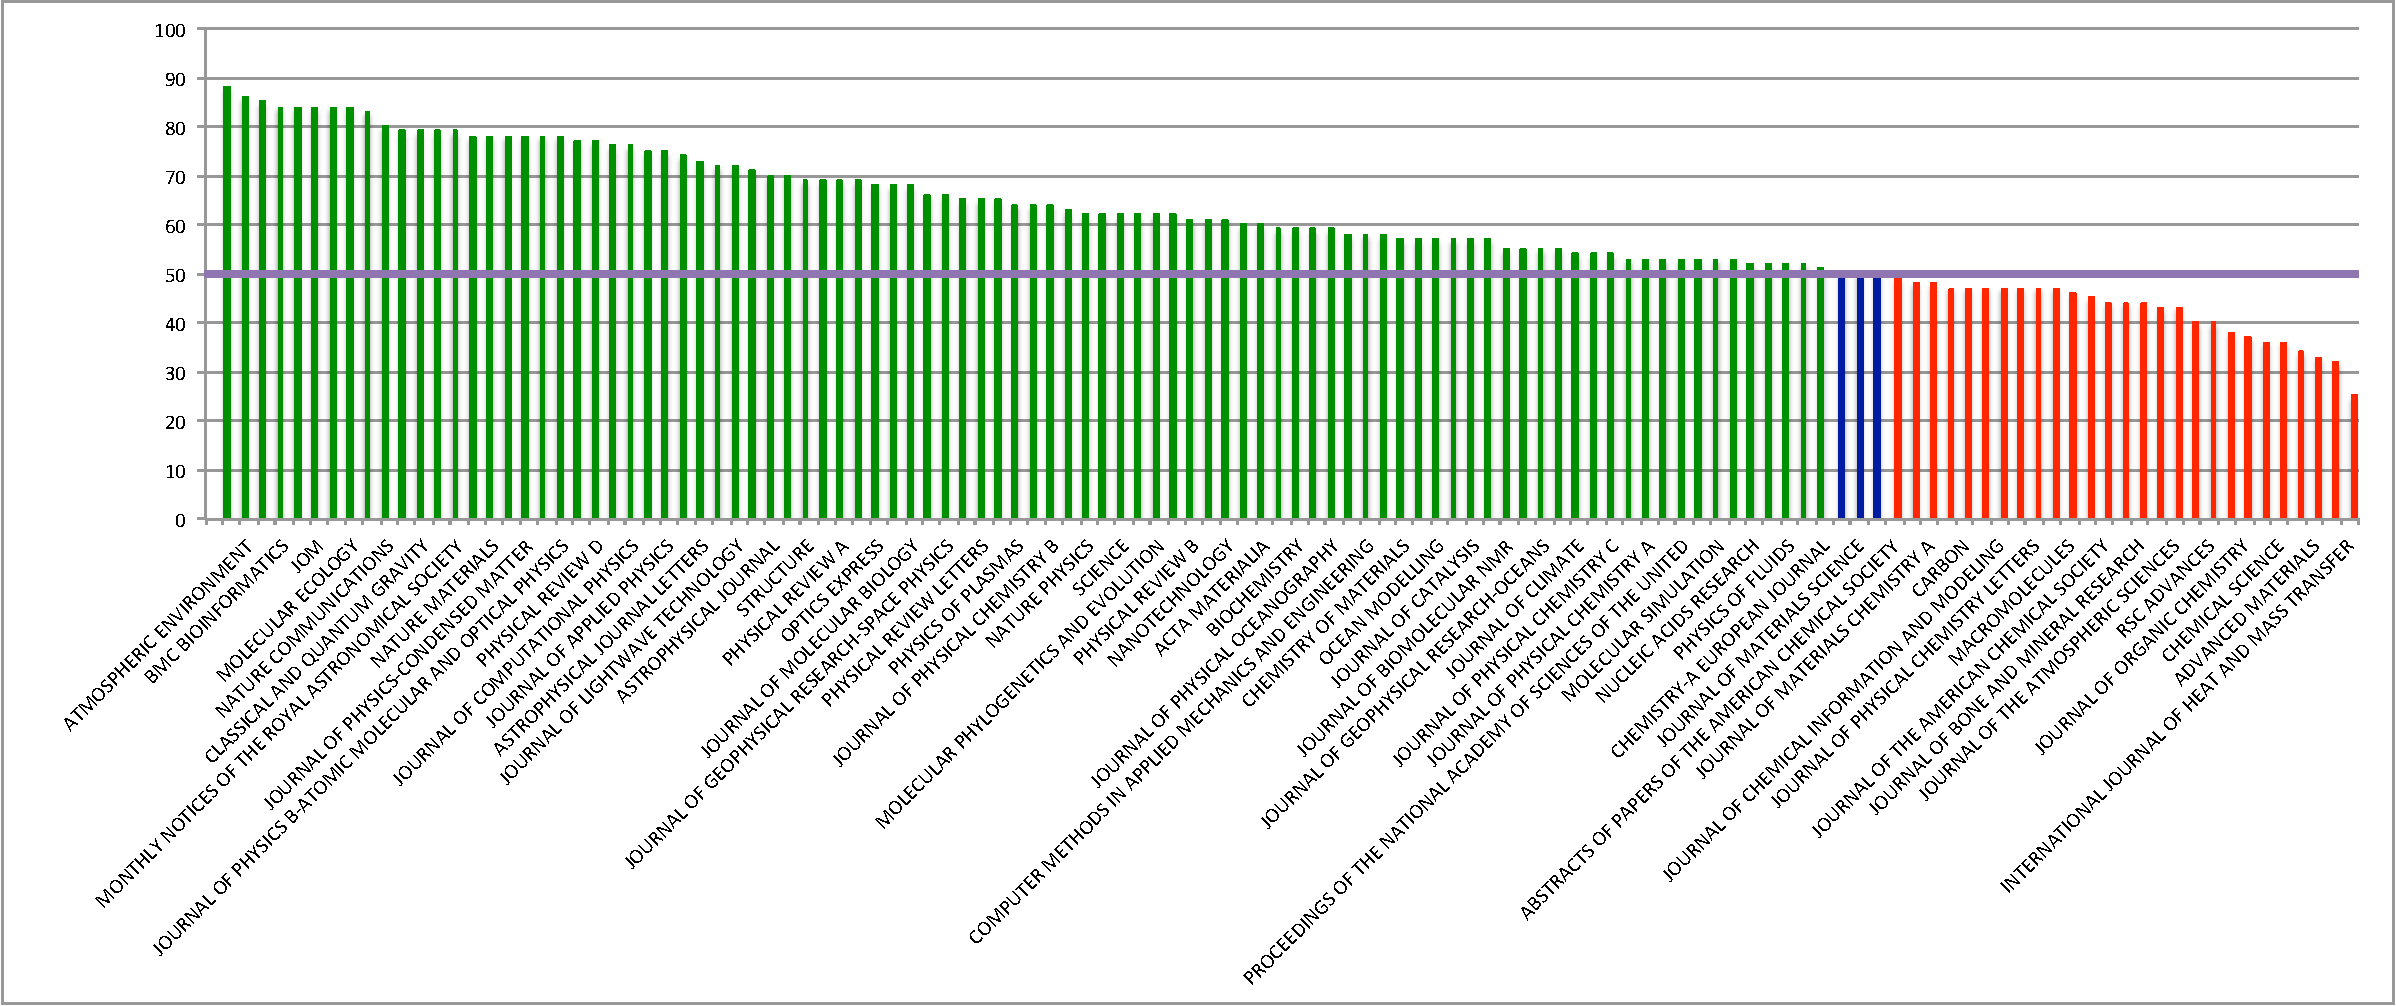
\includegraphics[width=0.9\textwidth]{images/isi_peers_byj_median.pdf}
    \caption{Median percentile ranking of XD publications by journal (by ISI)}
    \label{F:isi_peers_byj_median}
\end{figure*}

When we aggregate the results by fields of study instead of by
individual journal, we get the results shown in Figure~\ref{F:isi_peers_fos}.

\begin{figure*}[htb!]
  \centering
    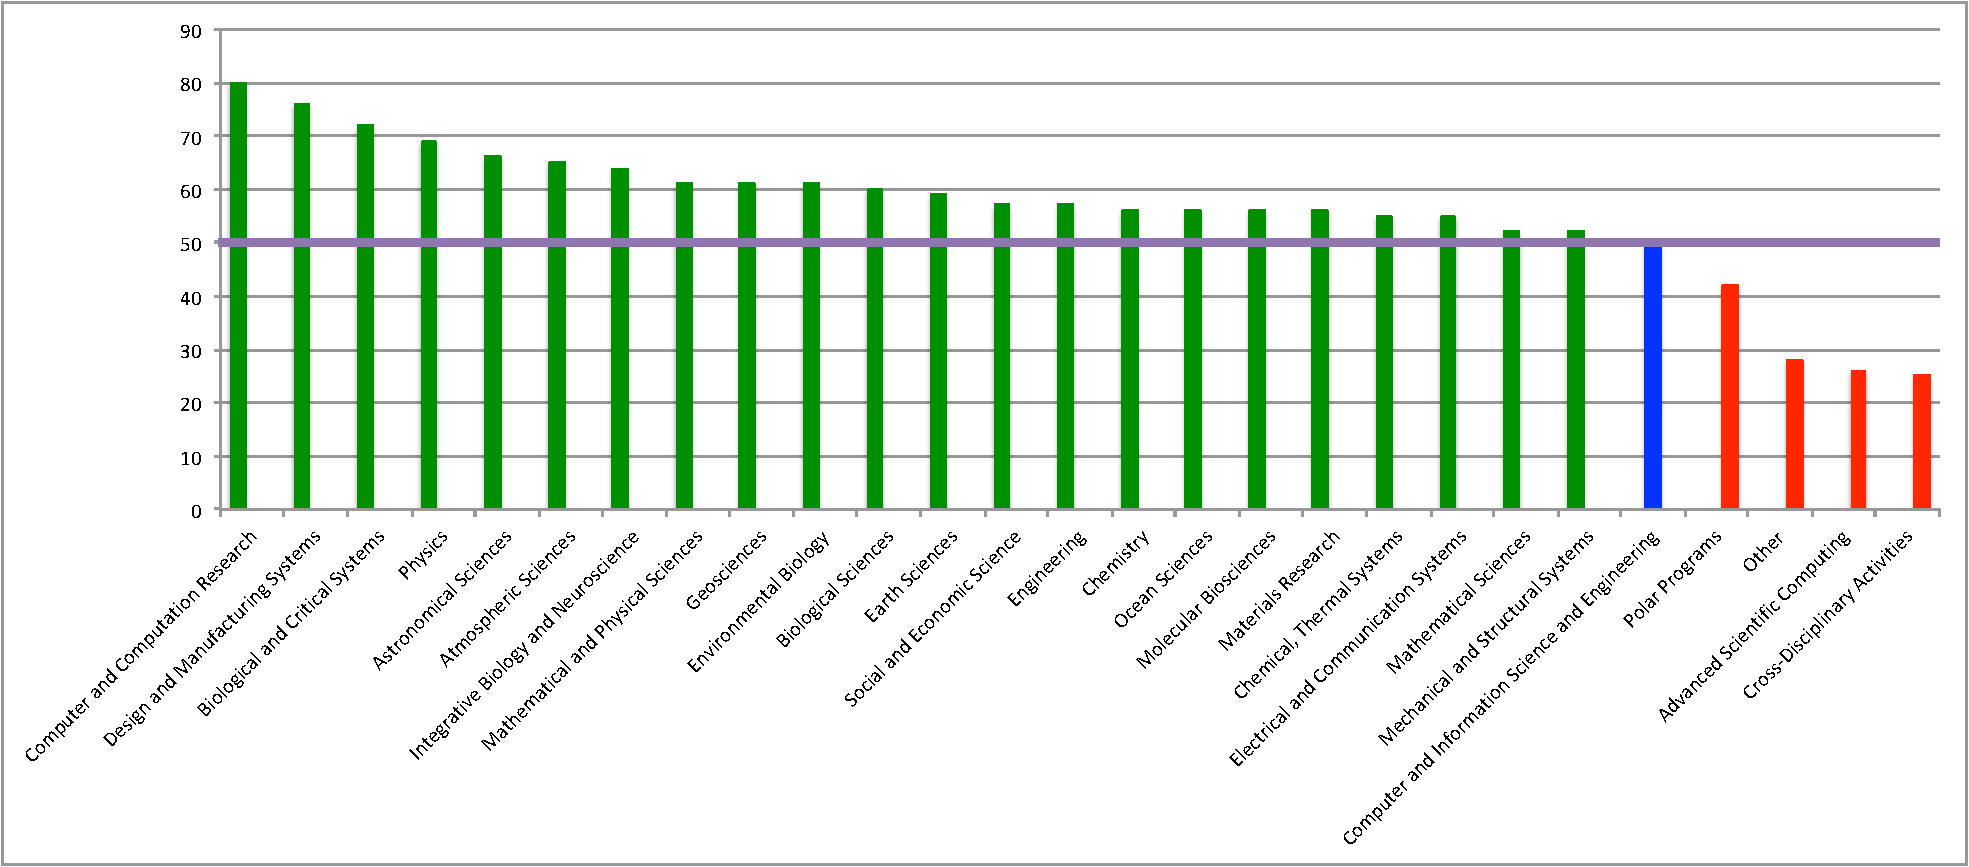
\includegraphics[width=0.9\textwidth]{images/isi_peers_fos.pdf}
    \caption{Average percentile ranking of XD publications by Field of Study (by ISI)}
    \label{F:isi_peers_fos}
\end{figure*}

These plots show that for majority of the publications venues, or fields of
science, XSEDE publications have a higher percentile ranking based on
citation count.

When we consider the overall comparison results,
Figure~\ref{F:ptranking_hist} shows the distribution of the XSEDE
publication's percentile rank in each 10\% increment group. Values
above 50\% indicate that the XSEDE publications are cited at a higher
rate than their non-XSEDE peers.  Again the result show the
distribution skewed to the higher end, which means that XSEDE
publications are cited more frequently than their non-XSEDE peers.

\begin{figure}[htb!]
    \centering
    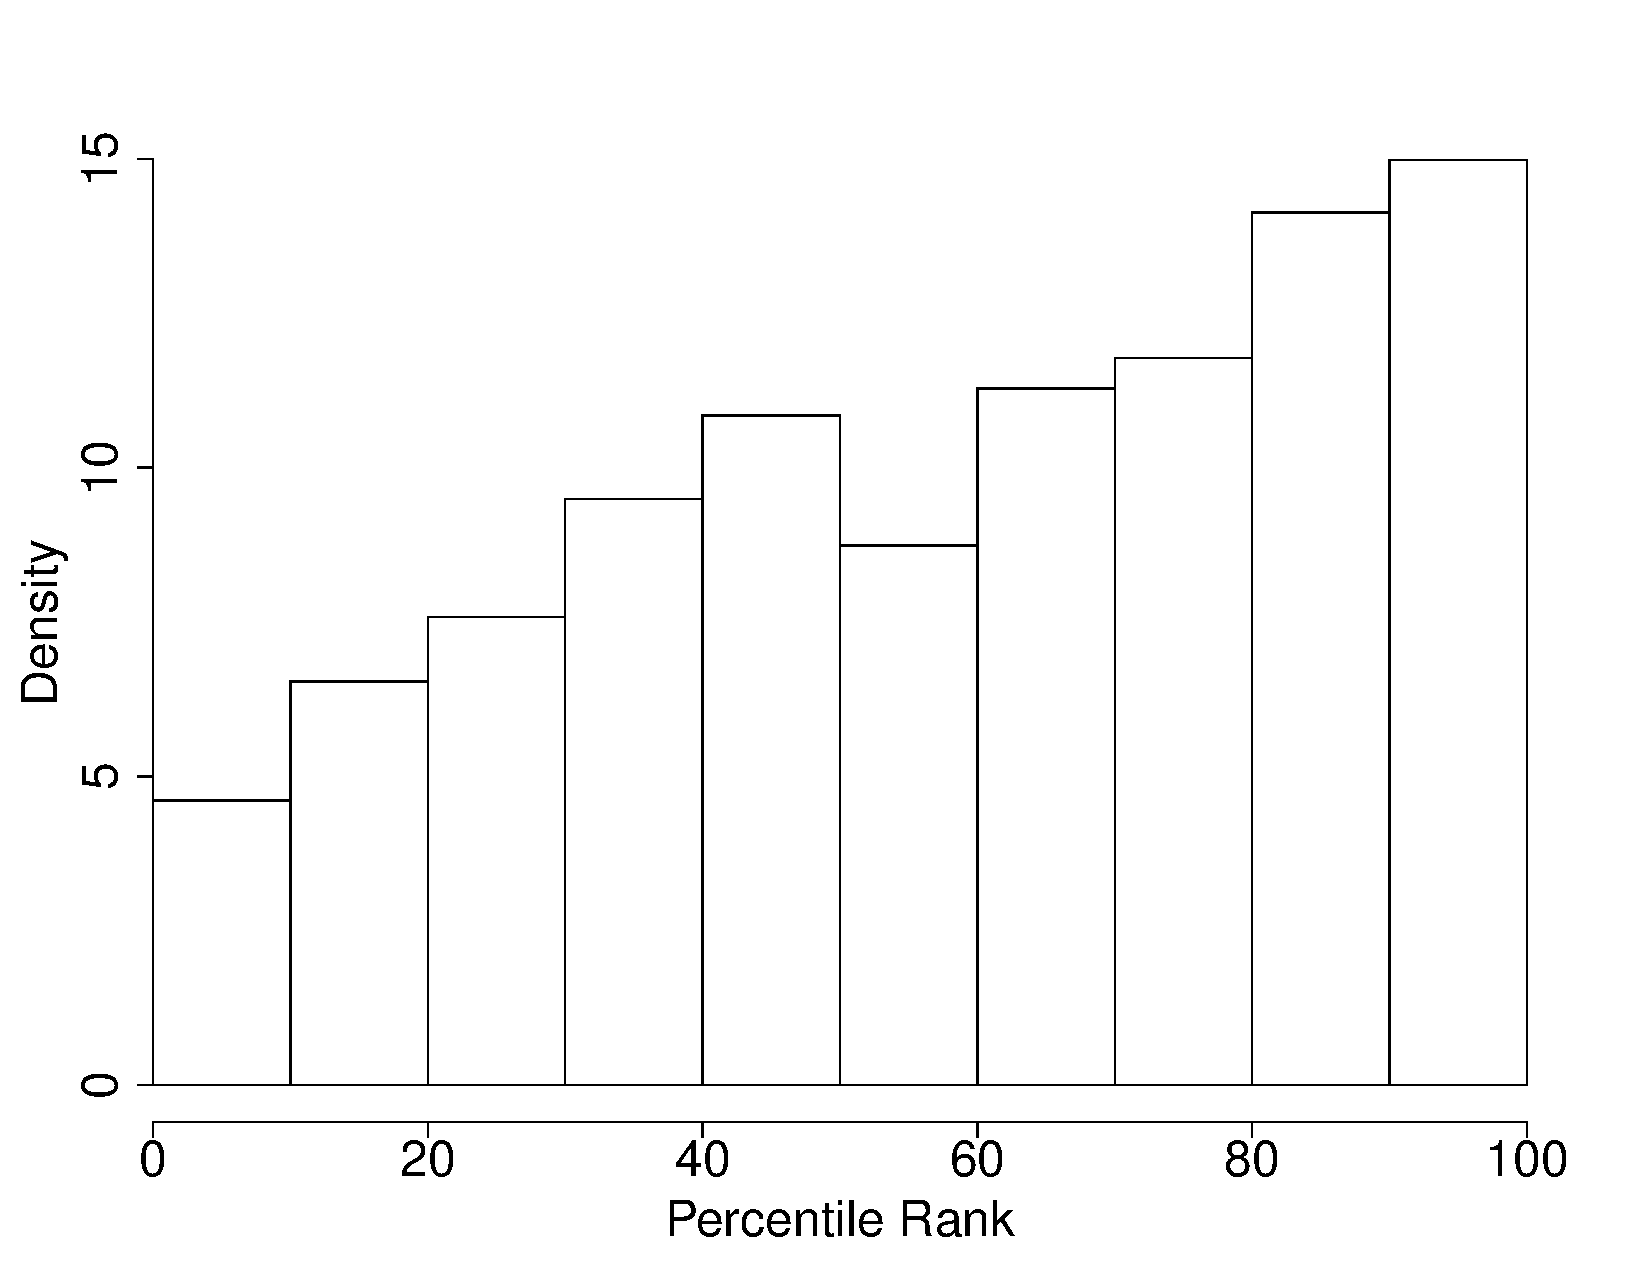
\includegraphics[width=0.80\columnwidth]{images/ptranking_histogram.pdf}
    \caption{Histogram of Percentile Ranking}
    \label{F:ptranking_hist}
\end{figure}

Figure \ref{F:ptranking_cdf} shows the empirical cumulative
distribution of the percentile ranks compared to that of the peers
group. The XSEDE publication curve is entirely to the right of the
overall publication curve which is another indication that the XSEDE
publications have a higher impact.  Figure~\ref{F:xd_peers_density}
shows the kernel density of the distributions of XSEDE publications'
percentile ranking and that of peers'. As expected, the non-XSEDE peer
publications are evenly distributed by percentile ranks with the spike
at 50\% mostly coming from more recently published journal issues
where most publications were not yet cited. The XSEDE publications are
weighted to the higher percentile ranks side again. This again shows
that XSEDE publications tend to be more highly cited compared to their
peers published in the same journal issue.

\begin{figure}[htb!]
    \centering
    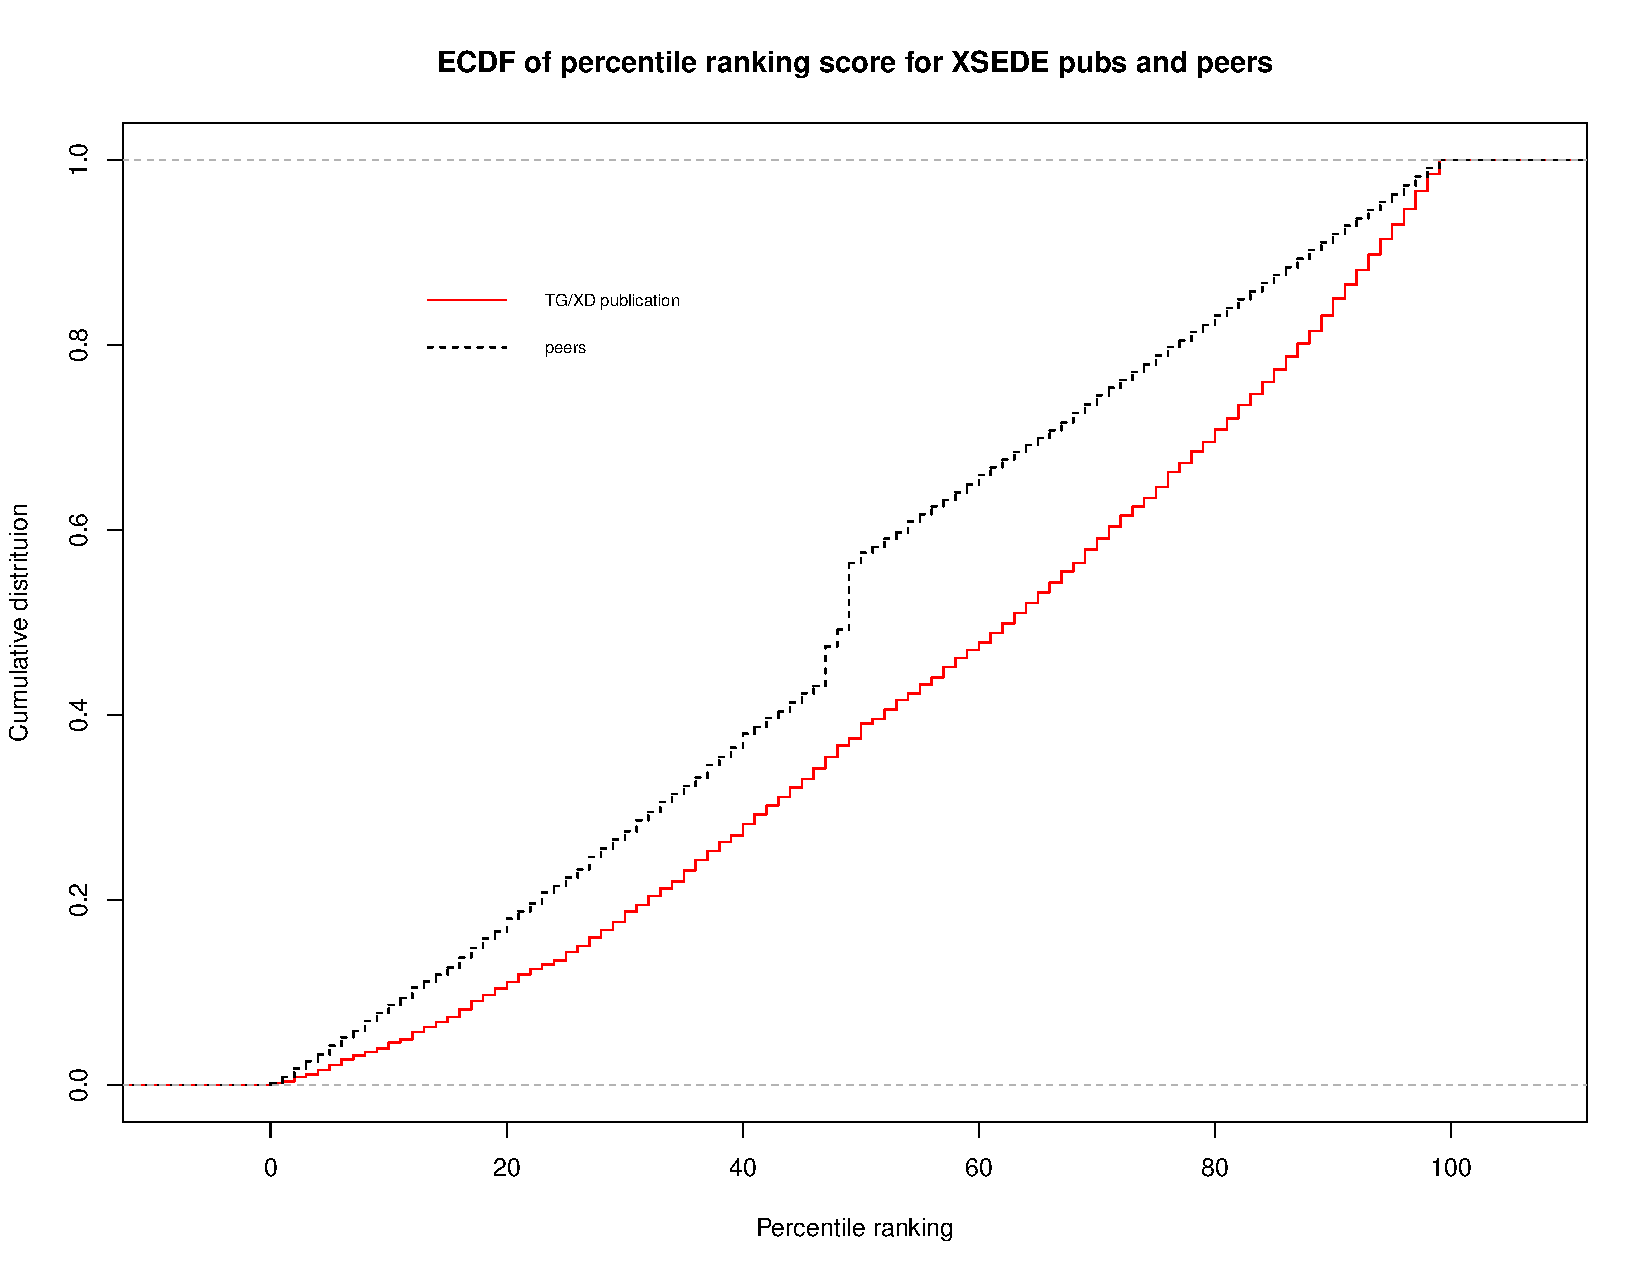
\includegraphics[width=0.80\columnwidth]{images/ptranking_CDF.pdf}
    \caption{Empirical Cumulative Distribution of Percentile Ranks}
    \label{F:ptranking_cdf}
\end{figure}

\begin{figure}[htb!]
    \centering
    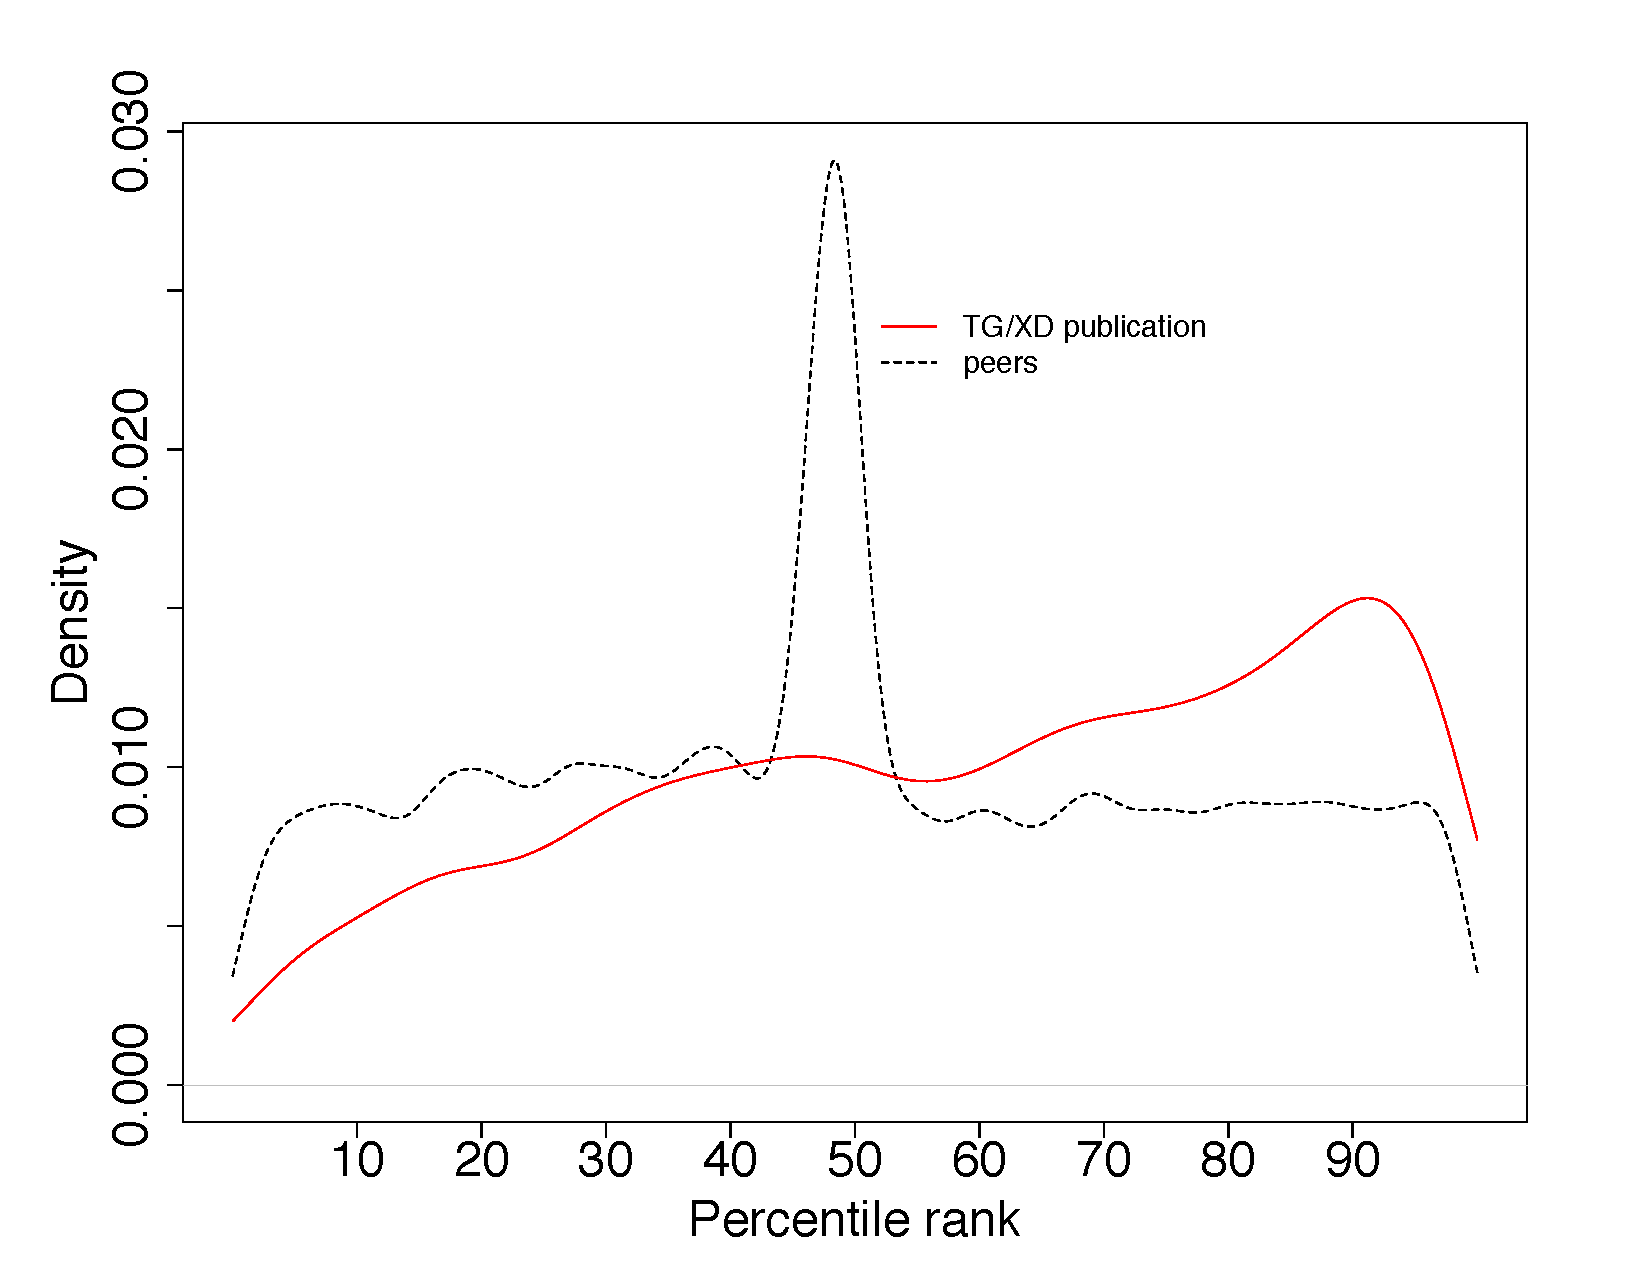
\includegraphics[width=0.80\columnwidth]{images/ptranking_distribution.pdf}
    \caption{Kernel Density of the distributions
of XSEDE publications' percentile ranking and that of peers'}
    \label{F:xd_peers_density}
\end{figure}

Table \ref{T:groups_stats} lists the average and median rankings and
citations received by XSEDE and non-XSEDE peer publication groups.

\begin{table}[h!]
\caption{Basic statistics of XSEDE publications group and peers group}
\label{T:groups_stats}
\centering
\resizebox{0.8\columnwidth}{!}{%
\begin{tabular}{lrrrrrr}
 & Number of & \multicolumn{2}{ c }{Rank} & \multicolumn{2}{ c }{Citations}  \\
 &  Publications & Average & Median & Average & Median \\
\hline
  XD     & 5078            & 59   & 63   & 28   & 12 \\
Peers & 356464 & 49   & 49   & 15   & 5 \\
\end{tabular}
}
\end{table}

We used several non-parametric statistical tests to decide whether the
XSEDE and non-XSEDE population distributions are identical without
assuming that they follow a normal distribution.  We used the
Mann-Whitney-Wilcoxon test~\cite{mann1947test}, Mood's median
test~\cite{brown1951median}, and Kruskal-Wallis
test~\cite{kruskal1952use}. The results are as the following.

Wilcox test for citation count
\begin{itemize}
\item W = 1160300000, p-value < 2.2e-16. Alternative hypothesis: true location shift is not equal to 0
\end{itemize}

Wilcox test for percentile ranking
\begin{itemize}
\item W = 1090700000, p-value < 2.2e-16. Alternative hypothesis: true location shift is not equal to 0
\end{itemize}

Mood's median test for citation count
\begin{itemize}
\item p-value = 3.299883e-172
\end{itemize}

Mood's median test for percentile ranking
\begin{itemize}
\item p-value = 8.83052e-71
\end{itemize}

Kruskal-Wallis Test for citation count
\begin{itemize}
\item Kruskal-Wallis chi-squared = 1207.6, df = 1, p-value < 2.2e-16
\end{itemize}

Kruskal-Wallis Test for percentile ranking
\begin{itemize}
\item Kruskal-Wallis chi-squared = 632.35, df = 1, p-value < 2.2e-16
\end{itemize}

All of these results strongly indicate that the differences that we
see between the XSEDE and the non-XSEDE publication metrics are
statistically significant.

We also performed a T-test to test the citation count differences and
percentile rank differences. Even though the distribution of the
citation count of the XSEDE publication group and the peers group are
not necessarily normally distributed, due to the central limit
theorem, when the sample size is large enough, it is rational to use
the T-test to not only test if there is a statistical difference
between the two groups, as having been shown by the several previous
tests, but also to quantify the difference between the means. The
t-test results for both citation count and percentile ranking are
given below.

\begin{itemize}
\item T=9.8328, df=5105.5, p-value< 2.2e-16, 95\% confidence interval: $[10.90, 16.32]$
\end{itemize}

T-test for ranking (Welch Two sample t-test)
\begin{itemize}
\item T=25.412, df=5105.5, p-value<2.2e-16, 95\% confidence interval: $[9.07, 10.59]$
\end{itemize}


The results show that the XSEDE group has a statistically higher
citation ranking and a statistically higher mean citation rate than
the non-XSEDE peer group.

\subsubsection{Journal peer comparison based on MAG data}

Although we first integrated the MAG data in order to evaluate the
field weighed impact of the XSEDE publications, we can follow the same
approach as was done using the WoS data to conduct a similar peer
comparison study. Figure \ref{F:ms_peers_byj_mean} and Figure
\ref{F:ms_peers_byj_median} show the average and median percentile
ranking for XSEDE publications by each journal using MAG data. The
overall results are pretty similar to what we got from the study with
the WoS data.

\begin{figure*}[htb!]
  \centering
    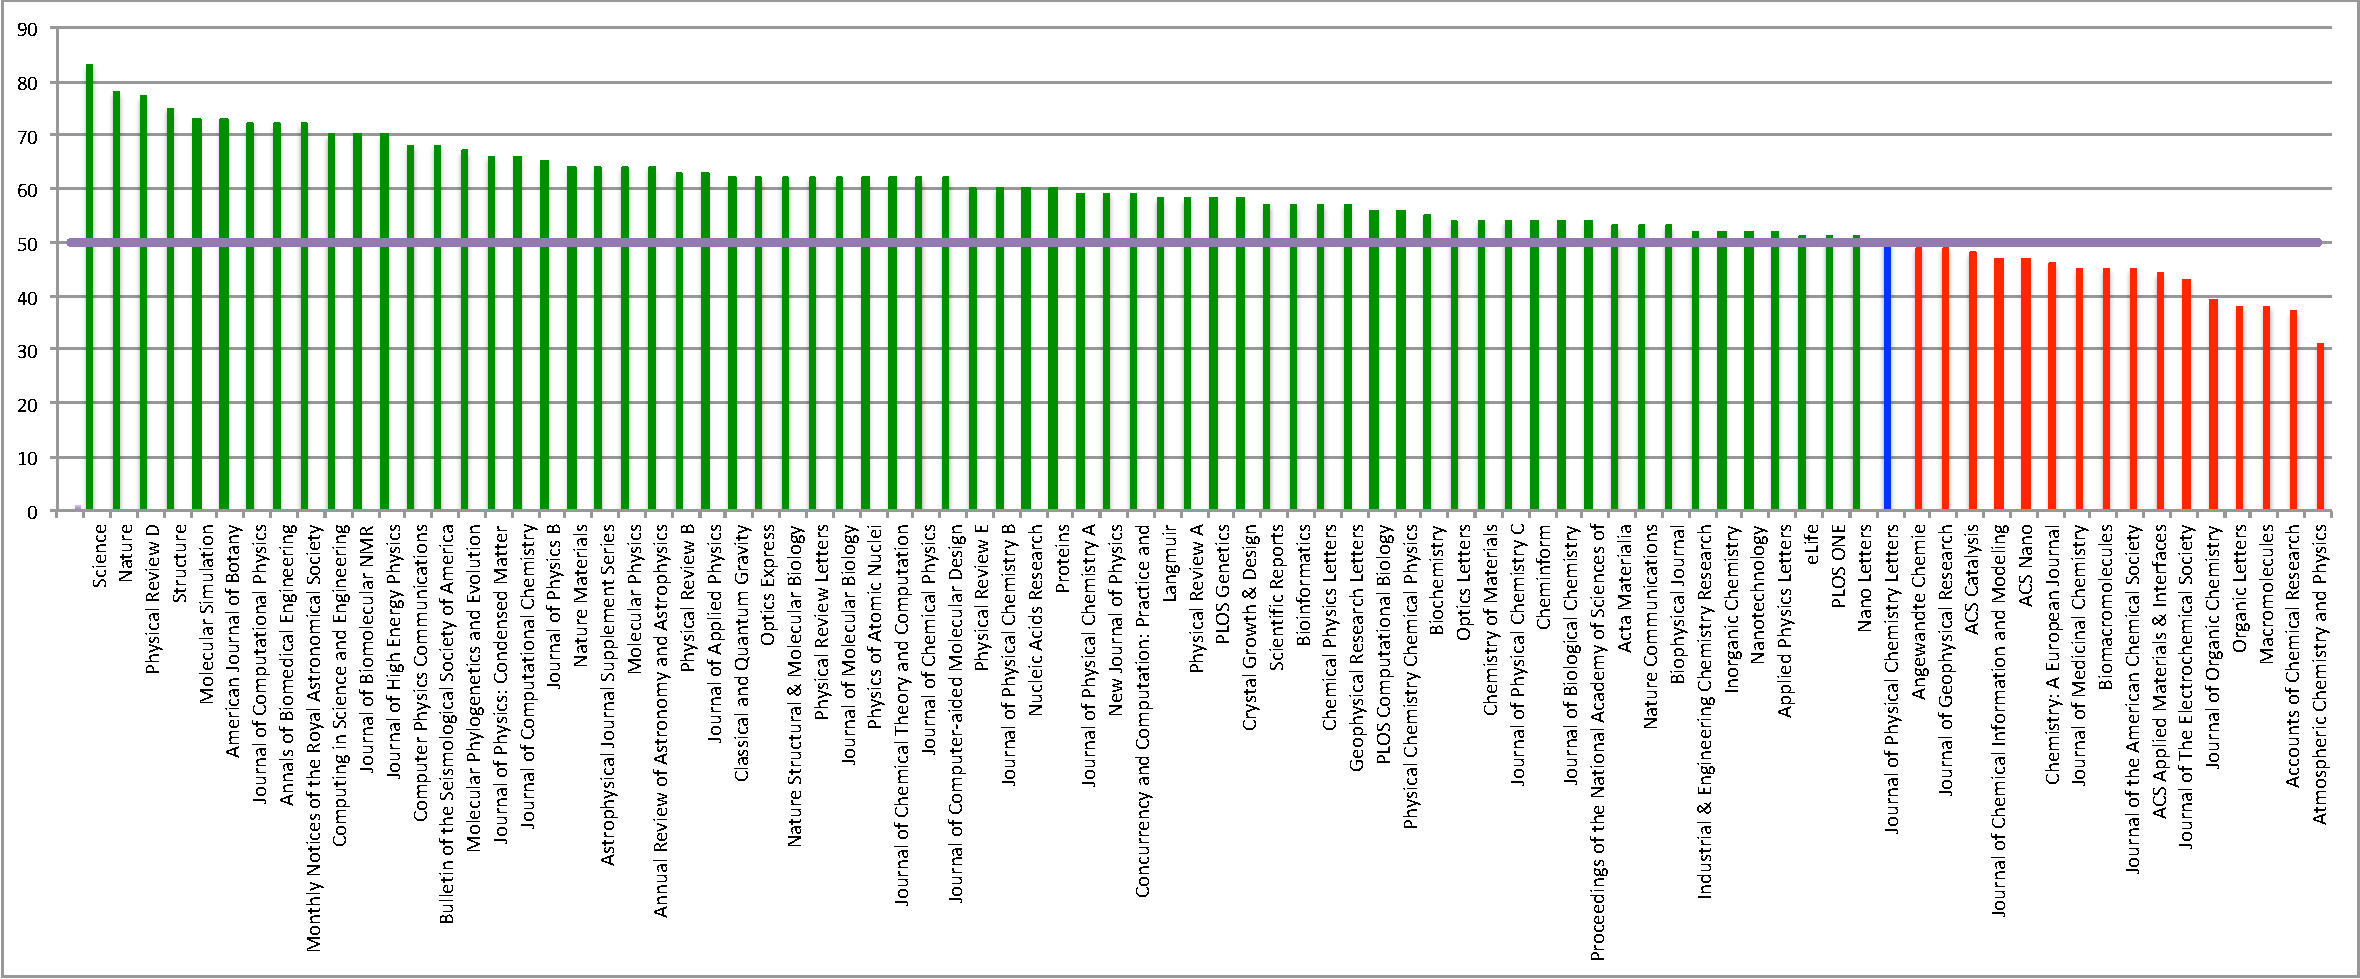
\includegraphics[width=0.9\textwidth]{images/ms_peers_byj_mean_10.pdf}
    \caption{Average percentile ranking of XD publications by journal (by MS)}
    \label{F:ms_peers_byj_mean}
\end{figure*}

\begin{figure*}[htb!]
  \centering
    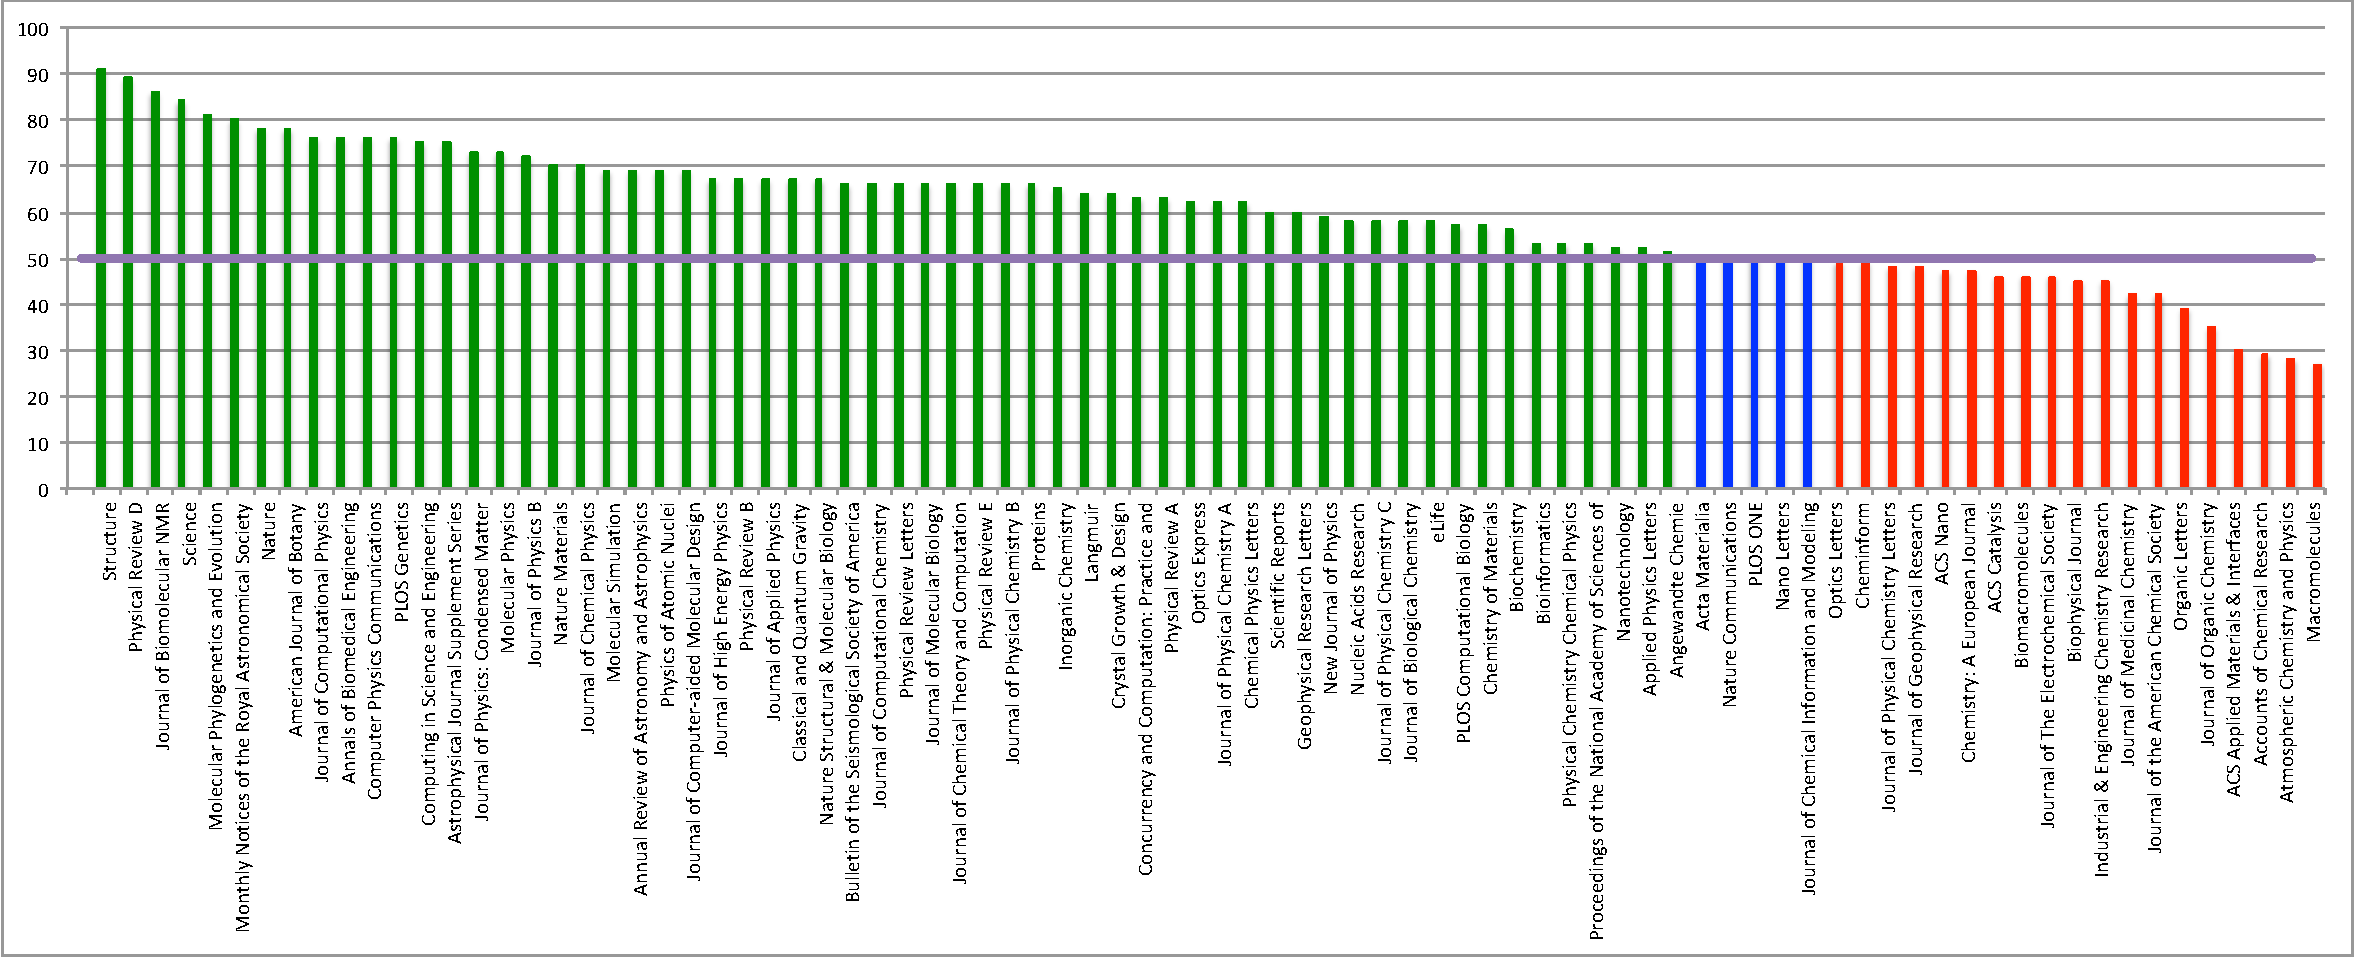
\includegraphics[width=0.9\textwidth]{images/ms_peers_byj_median_10.pdf}
    \caption{Median percentile ranking of XD publications by journal (by MS)}
    \label{F:ms_peers_byj_median}
\end{figure*}

\section{Conclusion} \label{S:conclusion}

We evaluated the scientific impact of XSEDE by examining the
publications that were enabled by having access to the XSEDE
resources. By curating the XSEDE publication data including cleansing,
verifying and correlating the various data sources, we obtained a
substantial very valuable dataset with which to compare and evaluate
the scientific impact of XSEDE itself.  While using two distinct
analyses - \emph{Field Weighted Citation Impact} analysis, and another novel
\emph{Journal Publications-based Peer Comparison} study, we found that XSEDE
publications tend to be cited more than non-XSEDE publications.
Various statistical tests show the results are statistically
significant.  The results from this study could potentially be used to
inform to the XSEDE leadership team and the funding agency about the
management of the facility, for example, to provide useful information
to the resource allocation committee during proposal selection and
approval.  While the present study dealt exclusively with XSEDE data,
the approaches and methods developed can be applied to evaluate
publication data from a variety of different facilities or groups.  In
fact we have done similar analyses for NCAR, BlueWaters, and Bridges
using the developed methodology and software framework.

%%%%%%%%%%%%%%%%%%%%%%%%%%%%%%%%%%%%%%%%%%%%%%%%%%%%%%%%%%%%%%%%%%%%%%
% Acknowledgment
%%%%%%%%%%%%%%%%%%%%%%%%%%%%%%%%%%%%%%%%%%%%%%%%%%%%%%%%%%%%%%%%%%%%%%

\section{Acknowledgments}

This work is part of the XSEDE Metrics Service (XMS) project sponsored
by NSF under grant number OCI-1025159. Lessons learned from FutureGrid
have significantly influenced this work. Gathering publications was
first pioneered by FutureGrid, influencing the development in the XSEDE
portal. We would like to thank Matt Hanlon and Maytal Dahan for their
efforts to integrate part of the services into the XSEDE portal.


\bibliographystyle{abbrvurl}
\bibliography{%
bib/tas,%
bib/vonlaszewski-new}


\end{document}

%%%%%%%%%%%%%%%%%%%%%%%%%%%%%%%%%%%%%%%%%%%%%%%%%%%%%%%%%%%%%%%%%%%%%%
%%%%%%%%%%%%%%%%%%%%%%%%%%%%%%%%%%%%%%%%%%%%%%%%%%%%%%%%%%%%%%%%%%%%%%
%%%%%%%%%%%%%%%%%%%%%%%%%%%%%%%%%%%%%%%%%%%%%%%%%%%%%%%%%%%%%%%%%%%%%%

% END END

%%%%%%%%%%%%%%%%%%%%%%%%%%%%%%%%%%%%%%%%%%%%%%%%%%%%%%%%%%%%%%%%%%%%%%
%%%%%%%%%%%%%%%%%%%%%%%%%%%%%%%%%%%%%%%%%%%%%%%%%%%%%%%%%%%%%%%%%%%%%%
%%%%%%%%%%%%%%%%%%%%%%%%%%%%%%%%%%%%%%%%%%%%%%%%%%%%%%%%%%%%%%%%%%%%%%

